%to have line numbers
%\RequirePackage{lineno}
\documentclass[10pt, letterpaper]{article}      
\usepackage[margin=.1cm,font=small,labelfont=bf]{caption}[2007/03/09]
%\usepackage{endnotes}
%\let\footnote=\endnote
\usepackage{setspace}
\usepackage{longtable}                        
\usepackage{anysize}                          
\usepackage{natbib}                           
%\bibpunct{(}{)}{,}{a}{,}{,}                   
\bibpunct{(}{)}{,}{a}{}{,}                   
\usepackage{amsmath}
\usepackage[% draft,
pdftex]{graphicx} %draft is a way to exclude figures                
\usepackage{epstopdf}
\usepackage{hyperref}                             % For creating hyperlinks in cross references


% \usepackage[margins]{trackchanges}

% \note[editor]{The note}
% \annote[editor]{Text to annotate}{The note}
%    \add[editor]{Text to add}
% \remove[editor]{Text to remove}
% \change[editor]{Text to remove}{Text to add}

%TODO make it more standard before submission: \marginsize{2cm}{2cm}{1cm}{1cm}
\marginsize{1cm}{1cm}{.5cm}{.5cm}%{left}{right}{top}{bottom}   
					          % Helps LaTeX put figures where YOU want
 \renewcommand{\topfraction}{1}	                  % 90% of page top can be a float
 \renewcommand{\bottomfraction}{1}	          % 90% of page bottom can be a float
 \renewcommand{\textfraction}{0.0}	          % only 10% of page must to be text

 \usepackage{float}                               %latex will not complain to include float after float

\usepackage[table]{xcolor}                        %for table shading
\definecolor{gray90}{gray}{0.90}
\definecolor{orange}{RGB}{255,128,0}

\renewcommand\arraystretch{.9}                    %for spacing of arrays like tabular

%-------------------- my commands -----------------------------------------
\newenvironment{ig}[1]{
\begin{center}
 %\includegraphics[height=5.0in]{#1} 
 \includegraphics[height=3.3in]{#1} 
\end{center}}

 \newcommand{\cc}[1]{
\hspace{-.13in}$\bullet$\marginpar{\begin{spacing}{.6}\begin{footnotesize}\color{blue}{#1}\end{footnotesize}\end{spacing}}
\hspace{-.13in} }

%-------------------- END my commands -----------------------------------------



%-------------------- extra options -----------------------------------------

%%%%%%%%%%%%%
% footnotes %
%%%%%%%%%%%%%

%\long\def\symbolfootnote[#1]#2{\begingroup% %these can be used to make footnote  nonnumeric asterick, dagger etc
%\def\thefootnote{\fnsymbol{footnote}}\footnote[#1]{#2}\endgroup}	%see: http://help-csli.stanford.edu/tex/latex-footnotes.shtml

%%%%%%%%%%%
% spacing %
%%%%%%%%%%%

% \abovecaptionskip: space above caption
% \belowcaptionskip: space below caption
%\oddsidemargin 0cm
%\evensidemargin 0cm

%%%%%%%%%
% style %
%%%%%%%%%

%\pagestyle{myheadings}         % Option to put page headers
                               % Needed \documentclass[a4paper,twoside]{article}
%\markboth{{\small\it Politics and Life Satisfaction }}
%{{\small\it Adam Okulicz-Kozaryn} }

%\headsep 1.5cm
% \pagestyle{empty}			% no page numbers
% \parindent  15.mm			% indent paragraph by this much
% \parskip     2.mm			% space between paragraphs
% \mathindent 20.mm			% indent math equations by this much

%%%%%%%%%%%%%%%%%%
% extra packages %
%%%%%%%%%%%%%%%%%%

\usepackage{datetime}


\usepackage[latin1]{inputenc}
\usepackage{tikz}
\usetikzlibrary{shapes,arrows,backgrounds}


%\usepackage{color}					% For creating coloured text and background
%\usepackage{float}
\usepackage{subfig}                                     % for combined figures

\renewcommand{\ss}[1]{{\colorbox{blue}{\bf \color{white}{#1}}}}
\newcommand{\ee}[1]{\endnote{\vspace{-.10in}\begin{spacing}{1.0}{\normalsize #1}\end{spacing}\vspace{.20in}}}
\newcommand{\emd}[1]{\ExecuteMetaData[/tmp/tex]{#1}} % grab numbers  from stata

%TODO before submitting comment this out to get 'regular fornt'
\usepackage{sectsty}
\allsectionsfont{\normalfont\sffamily}
\usepackage{sectsty}
\allsectionsfont{\normalfont\sffamily}
\renewcommand\familydefault{\sfdefault}

%\usepackage[margins]{trackchanges}
\usepackage{rotating}
\usepackage{catchfilebetweentags}

\usepackage{abstract}
\renewcommand{\abstractname}{}    % clear the title
\renewcommand{\absnamepos}{empty} % originally center
%-------------------- END extra options -----------------------------------------
\date{{}\today}
\title{  
The effect of social transfers and social capital on subjetive wellbeing of
elderly\footnote{This study was funded by grant \# 2016/21/B/HS4/03058 from
  Polish National Science Foundation (Narodowe Centrum Nauki).}
}
\author{
% Adam Okulicz-Kozaryn\thanks{EMAIL: adam.okulicz.kozaryn@gmail.com
%   \hfill I thank XXX.  All mistakes are mine.} \\
% {\small Rutgers - Camden  and Vistula University}
% and Leszek Morawski\thanks{EMAIL: l.morawski@vistula.edu.pl}\\
% {\small Polish Academy of Sciences and Vistula University}
}

\begin{document}

%%\setpagewiselinenumbers
%\modulolinenumbers[1]
%\linenumbers

\bibliographystyle{/home/aok/papers/root/tex/ecta}
\maketitle
\vspace{-.4in}
\begin{center}

\end{center}


\begin{abstract}
\noindent We investigate the effect of social transfers (especially pension) and
social capital (especially volunteering) on subjective wellbeing (SWB) of
elderly using the latest wave 6 of Survey of Health, Aging and Retirement in Europe
(SHARE). We find that the effect of volunteering on SWB is not much smaller or
even about as large as that of pensions. The most SWB is associated with volunteering about
every week, but there is already a substantial effect even if one volunteers only
about every month. 
We also find that the higher the income or wealth, but not pension, the lower
the effect of volunteering.  
High European pensions may be unsustainable in the long run--we argue that
 promotion of volunteering is one way to increase elderly's subjective wellbeing amidst tightening budgets.
\end{abstract}
\vspace{.15in} 
\noindent{\sc Subjective Wellbeing (SWB), Life Satisfaction, Happiness, Aging,
  Elderly, Volunteering, Social Transfers, Social Capital, Survey of Health, Ageing and Retirement in Europe (SHARE) 
}
\vspace{.25in} 

\begin{spacing}{1.4} %TODO MAYBE before submission can make it like 2.0
\rowcolors{1}{white}{gray90}

%  instead \ExecuteMetaData[../out/tex]{ginipov} do \emd{ginipov}

% \begin{figure}[H]
%  \includegraphics[height=3in]{../out/gov_res_trust.pdf}\centering\label{gov_res_trust}
% \caption{woo}
% \end{figure}


Population aging will be the key issue in this century, and perhaps even in 
the third
millennium  \citep{stolnitz1992demographic}. Specifically, there are growing
concerns about sustainability of pensions and health care \citep{jurges12}. 
The problem of aging is clear in many European countries, e.g., in
Germany, Europe's most populous country, and there is clearly a need for social
science research to address aging as one of the most important challenges of our
times \citep{vaupel2006redistributing}. 
%
Amidst growing concerns about sustainability of pensions and health care, there
is much need to investigate alternative ways  of sustaining and increasing  the wellbeing of
the elderly. % and what are the tradeoffs.
 In present study % predicting SWB
we are especially interested in whether the effect of volunteering is comparable
to that of pensions. In other words, we
study how much SWB is dervied from economic v social capital. 
% substitution between economic
% capital (social transfers) v social capital (volunteering).
% latest: AH NOT SURE NOT REALLY DOINGH ANY SUBSTITUTION TEST OR ANYTHING,
% rather just simply a net effect
% MAYBE use this terminology more;
                                %definietly at least one more guess at the end
%collective social policy and individual believes/values.
%  We will also control for a number of person-level characteristics.
%Our audience is broad--anybody interested in well-being and quality of life.

Volunteering has been advocated by the United Nations, American and European
governments as a way to engage people in their local communities and improve
social capital, with the potential for public health benefits such as improved 
health and overall wellbeing 
\citep{jenkinson2013volunteering}. Promotion of volunteering could be an
alternative 
strategy to sustained social transfers in an effort to achieve a decent
wellbeing.  For other strategies see \citet[][sec. 2.4.5]{ferring10}. 

There is a need for new knowledge: better understanding of the determinants of
SWB enables to evaluate and possibly reform present retirement
institutions, such as pension programs, as well
as potentially generate new institutions to meet the demands of rapidly
increasing retirement population. SWB can serve as a yardstick to evaluate
relative strength and net effect from each factor. In present study, we will use SWB
to measure net effects of social transfers and social capital--we will control
for both in one model.

There is a growing recognition of subjective  well-being and quality of life
indicators \citep{aok_lsPol16}. Traditional
measures of development, such as income, production, or consumption are too
simplistic. They do not capture the overall progress of our civilization. For
instance, gross domestic product increases when there is traffic congestion, but
clearly that is not 
progress. But even increase in household income does not necessarily
 create progress if there is growing income inequality. 
Other important ingredients of overall development and progress such as
discretionary time, mental and physical health are not captured by monetary measures. We will
capture overall progress by using SWB yardstick.

%
 % Research focusing on aging and happiness takes into account income, but either
 % overlooks social transfers or volunteering or both.
 We start with a general hypothesis about social
 transfers and social capital, which is multi-dimensional, and we focus  on volunteering:\\
\noindent$H_1:$ The more social transfers and social capital, especially in the
form of volunteering, the more SWB.\\

Studies focusing on elderly and their wellbeing, either miss social
transfers or volunteering (they do not examine them simultaneously), and they
often measure only specific domains of wellbeing, not overall wellbeing. We
hypothesize some degree of tradeoff or substitution between social capital and
social transfers. The more social capital, especially in the form of volunteering,
the lower the need for social transfers to achieve SWB.\\ 

\noindent$H_2:$ When considered simultaneously pensions and volunteering have about the same effect on SWB.\\ 

The above were our initial hypotheses we set off with for this project. In the
course of analysis, we have discovered an interaction between income, wealth, and
volunteering and we will report these results at the end. 

\section{SWB} 

SWB is multidimensional. Hedonic dimension is about prevalence of pleasure over
pain. Eudamonic dimension is about ``good life.'' There is affective momentary
happiness, and there is cognitive evaluative life satisfaction. There is some
overlap between the two, and there even more dimensions. Notably there are domain satisfactions:
community, financial, and so forth. For elaboration and discussion see \citet{diener09,diener04s,veenhoven08,kahneman99,campbell76etal}.

We will use two measures that are overall or all-inclusive, as opposed to
confined to a domain or domains, and are mostly cognitive and evaluative
as opposed to affective and momentary: single item life satisfaction question
and CASP scale \citep{hyde03,hyde15}. Life satisfaction is rather hedonic. CASP
scale is more comprehensive and includes some eudamonic items as discussed later.

CASP can be conceptualized as Control, Autonomy, Self-realization, and Pleasure \citep{hyde03,hyde15}.
CASP is often referred to as quality of life (QOL) measure, however, it is probably better understood as SWB measure--QOL measures are rather
objective \citep{aok13liavbility,aok-swbLivability18}. We also follow
\citet{vanhoutte12,vanhoutte14} who also considers CASP to be a SWB measure.

One could take volunteer process perspective and approach volunteering
as having antecedents, consequences, but also the middle category--the
experience of volunteering \citep{wilson12B}. We study here SWB as a consequence
of volunteering and our measures of SWB are well suited for it.

% While we specifically precisely mean life satisfaction, we also use a more
% generic term subjective wellbeing or even happiness. To be clear, we always mean
% overall life satisfaction, unless indicated otherwhise. For instance, we do not
% study here financial, community or other satisfactions. 

%SWB is our dependent variable.
%  SWB can be defined as people's evaluations of
% their lives, which include ``both cognitive judgments of one's life
% satisfaction in addition to affective evaluations of mood and
% emotions'' \citep{steel08}. In other words, it is ``overall judgment of life that draws on two sources of information:
%   cognitive comparison with standards of the good life (contentment) and
%   affective information from how one feels most of the time (hedonic
%   level of affect)'' \citep{veenhoven08}.  
 % Some scholars make a
%   distinction between happiness and life satisfaction. Life
%   satisfaction refers to cognition and happiness refers to affect \citep{dorahy98etal}. In practice, however, it is usually difficult
%     if not impossible to separate the two concepts. 
% Hence, the overall happiness definition by 
%    \citet{veenhoven08}, as quoted above,  seems most appropriate and we will use
%    terms ``subjective well-being (SWB),'' ``happiness,'' and ``life
%    satisfaction'' interchangeably. 

The SWB measures, even though self-reported and
 subjective, are  reliable (precision varies) % per ruut asa13 slides
 and valid \citep{myers00,ditella06m,diener09}. 


\section{Volunteering}

% focus on def of voluntering as among elderly
% Dictionary defines volunteering as
% definintion: voluntering: altruistic, etc
% \url{https://www.google.pl/search?q=volunteering+definition&rlz=1CATAAC_enUS742US743&oq=volunteering+definition&aqs=chrome..69i57j0l5.4820j0j7&sourceid=chrome&ie=UTF-8}
% The key of definition is altruism
\citet[][p.177]{wilson12B} provides a useful overview of definitions: 
%Snyder and Omoto  %from lm 
 define volunteering as
 ``freely chosen and deliberate helping activities that
extend over time, are engaged in without expectation of reward or other
compensation
and often through formal organizations, and that are performed on behalf of
causes or individuals who desire assistance.'' Another example of definition is ``unpaid help given
to another person not a member of one's family.'' The key part of definition is altruism.

Elderly are often an unused productive potential.
The literature agrees that volunteering is a productive aging strategy
\citep[e.g.,][]{wilson12B,hank09}. 
There is evidence that reward experienced from helping others may be deeply
ingrained in human nature, emerging in diverse cultural and economic contexts \citep{aknin13}.

\citet{anderson14} is a recent comprehensive review of benefits of
volunteering among seniors: volunteering is associated with reduced symptoms of
depression, better self-reported health, fewer functional limitations, and lower
mortality. The protective benefits associated with volunteering are amplified if
volunteers feel reciprocity (i.e., their work is appreciated and ``matters''), contribute their
time for prosocial reasons, and make a moderate but not excessive commitment to
volunteering. Indeed, volunteering can have negative effects, especially if done
in disaster situations (earthquakes, etc) or towards people in very difficult
situations (Ebola, etc) \citep{wilson12B}.

\citet{wilson12B} in his review lists many antecedents: again, volunteers report fewer depression symptoms. Volunteering
earlier in life predicts volunteering later in life and increased purpose in
life. It helps if one volunteers for extrinsic as opposed to intrinsic reasons. 
% Volunteering is likely to be overstated:  those who
% respond to surveys are more likely to volunteer, hence, actual volunteering in
% population is likely to be substantially lower. %p178


\section{Social Transfers}

%We know very little about the effect of social policy on wellbeing.
There is an abundant literature about the effect of welfare on SWB as recently
reviewed in \citet{aokJap14}. {Political scientists tend to focus on welfare and institutions at country
level \citep{alvarez09,pacek08b,radcliff13,pacek08r,radcliff01,bok10}. A popular
measure of welfare is a so called ``decommodification.'' % On the societal level, \citet[p. 36]{esping90} argued that ``the market becomes to the worker a prison within which it is imperative to
% behave as a commodity in order to survive.''
%  When workers feel like they are a commodity that leads to lower SWB \citep{easterlin09}.
% Additionally,  \citet{lane00} contended that  markets are indifferent
% to the fate of individuals so when there is not a safety net, people
% have lower SWB.  
Decommodification mostly means good pensions, sickness benefits,
and unemployment compensation--measurement is described in  \citet{scruggs06Ba}. Our approach is to zoom
in at person level and focus on elderly.} % There is even more research about the effect of personal income on
% happiness \citep{dolan08al,veenhoven12,helliwell14b}. 
% In general, both income and welfare increase SWB, at least up to a point. 
%
% Yet, there is clearly a gap: welfare is studied at aggregate level, usually 
% country level, and despite voluminous research linking income with SWB, there
% are very few studies about welfare or social transfers at person level, and
%  all these studies overlook social capital, notably volunteering. 
% BELOW MAYBE A FOOTNOTE TO FLOW BETTER
 There are surprisingly different relationships between SWB and its predictors
 depending on the level of analysis \citep{ashkanasy11}, and research implications can be
misguided when taken from only one level of analysis \citep{klein00}.

Many studies at person level focused on income and found that 
personal  income  increases SWB at least with diminishing returns
\citep{aok_ruut_inc_ine,kahneman10,frijters04,kushlev15,dolan08al,veenhoven12}. Yet,
this line of happiness research about personal income tends to overlook welfare
and social transfers--main reasons are probably twofold: researchers tend to
focus solely on income often following Easterlin paradox \citep{easterlin10B} and most data do
not allow for fine-grained measurement of social transfers or welfare. 
%
There are some exceptions. Notably, there is a recent experimental study \citep{oswald14}. Poor British
were given additional help from the government (training and money),  
were followed for several years, and at the end, the ones that received
additional welfare were not richer or happier than those who did not receive the
 help, if anything, they
were worse off. There is, however, no study considering simultaneously social transfers
including pensions and social capital including volunteering.

\section{Predicting SWB}

Our contribution is that we  investigate SWB among elderly
across multiple countries using large representative samples and focus on volunteering and social transfers simultaneously.  
%
Studies focusing on elderly and their wellbeing, either miss social
transfers or volunteering (they do not examine them simultaneously), and they
often measure only specific domains of wellbeing. For instance,
\citet{bender12} overlooks volunteering and studies retirement satisfaction: ``All in all,
would you say that your retirement has turned out to be very satisfying,
moderately satisfying, or not at all satisfying?''
% We have also looked at all studies that cite \citet{bender12}.
% Furtehrmore, his research  focuses on job satisfaction and uses data for the US only, and we focus
% on welfare, volunteering and study elderly in Europe. Furthermore his sample was
% restricted to individuals 51 to 61 years old, ours is 50$+$, and uses a sample
% of only about 6k people, and our sample is much larger. 
\citet{butrica2005satisfaction} also study retirement satisfaction, do focus on
volunteering (and interestingly suggest that volunteering in excess of 1k hours
per year does not help with satisfaction), but miss social transfers. All studies in a recent issue of Social Indicators Research \citep{jurges12} dedicated to aging and
wellbeing used other dependent variable than SWB, except one
\citep{angelini2012age}, which again, did not focus on social transfers and social capital/volunteering.
Studies that focus on happiness (SWB) and retirement also either miss social
transfers or volunteering
\citep{dingemans2014involuntary,dingemans2015retirement,nikolova2014employment,angelini2012age}.
 Many of such studies are more than ten years old and carried out in the US
\citep{wheeler98,ferring10}. % --older studies tend to use simpler methods, smaller samples, and fewer variables
%MAYBE:add more of this kind of lit
 Keep in mind that both volunteering and social transfers are very different in
 the US as compared to Europe \citep{tocqueville03,fischer10, alesina05al,alesina01,lipset00}.

%
 Volunteering predicts SWB. For a review see section 
 ``3.4.4. Community involvement and volunteering'' in \citet{dolan08al}. Cohort
 studies showed that volunteering had favorable effects on depression, life
 satisfaction, wellbeing but not on physical health \citep{jenkinson2013volunteering}.
%
What could be the causal pathway, how could volunteering cause SWB? Being a
volunteer transforms one's perceptions of herself, emotions, and knowledge of
the world \citep{wilson12B}. %p195
Volunteering boosts one's self esteem and buffers against stress, and
importantly it enhances mastery experiences
\citep{wilson12B}. %p198
%
 There is  some evidence of causal relationship between volunteering and
 happiness \citep{meier2008volunteering,borgonovi2008doing}. For instance, low status is associated
with low SWB only among those who do not volunteer--volunteering
might contribute to SWB by increasing empathy, shifting aspirations and by
moving the reference group to the relatively worse-off
\citep{borgonovi2008doing}. There are, of course, other causal pathways
possible. And we do not focus on causality in this correlational study.

Specifically, volunteering has been found to predict happiness among elderly (in
New Zealand) and the effect was moderated by
economic resources: poor benefit more from volunteering than rich
\citep{dulin2012volunteering}. And elderly benefit more than  younger people
\citep{van2000differential,wahrendorf06}. This may indicate that acting in
a social role beyond employment is beneficial for wellbeing.


\section{Data} 

We use the Survey of Health, Aging and Retirement in Europe (SHARE) from
\url{http://www.share-project.org}.
 SHARE is a multidisciplinary and
cross-national panel covering health, socio-economic status,
social and family networks of over 50,000 persons aged 50$+$. 
We use  %Wave 4 mostly in 2011
 Wave 6 releaase 6.0
 conducted  in 2015, which has the largest number of
countries of all waves. 
%
For robustness, we have also used wave 4 and obtained similar results--results
are available upon request.  


% On the other hand, 
An advantage of SHARE is few missing values, 
 and there is imputed dataset without any values missing (we collapse dataset--take an average across categories on implicat variable). %also representative at nuts1 i guess!

                                
Especially earlier waves have few countries--SHARE sample grew substantially
over time and its country coverage almost doubled. Another advantage of wave 6 is that
data were collected in just one year (2015), %; eg may be problem in debbie haski and otehrs
while in earlier waves data were collected over longer spans--seasonality may be
a problem in studies using earlier waves of the dataset.

Key variables are discussed below and all variables are listed in appendix along
with their distributions and module source.
Most of the variables are from the imputed module; we have used other modules
only when variable was not available in imputed module. For instance, social capital including
volunteering comes from Activities (AC) module. 

%  We use a number of restrictions to drop
% respondents who cannot volunteer or are severly restricted to do so based on the
% criteria defined below.
 We use MN and CF modules to
exclude elderly in retirement homes and proxy observations.
%
We drop people who were in nursing homes (\~\ 1\%): such persons typically do
not have opportunity for volunteering. We also drop proxy respondents and only retain
main participants (\~\ 5\%). %leszek
                                %says monika says that there is a way to drop
                                %proxies based on that verbal score 
% we exclude those in opieki spolecznej mn024--they cannot volunterr (about .3k dropped); and we drop
% proxies, and only retain main participants (about 1.5k dropped)
 We drop respondents younger than 50 (\~\ 2\%). % We drop
 % respondentd with restricted mobility ($>=5$ on variable mobility measuring arm
 % function and fine motor limitations).

%just use  aweights with calibrated weights--that's what michal myck says!
% yeah but emailed share and they say to used pw

All dollar amounts are PPP (Purchasing Power Parity) adjusted. We adjust all money amounts with
PPP--arguably what matters for SWB is rather what money buys not its numeric value.

%ESS happiness question reads: "All things considered, how satisfied are you with your life as a whole nowadays? Please answer using this card, where 0 means extremely dissatisfied and 10 means extremely satisfied."
SHARE contains typical life satisfaction question: %http://www.share-project.org/fileadmin/pdf_questionnaire_wave_4/SHARE_generic_wave4_main_questionnaire.pdf
``On a scale from 0 to 10 where 0 means completely dissatisfied and 10 means
completely satisfied, how satisfied
are you with your life?'' The survey-based life
 satisfaction measure is closely correlated with similar objective
 measures such as brain activity \citep{layard05}.
 We also use CASP scale to measure subjective
wellbeing. Life satisfaction and CASP are correlated at .6.  SHARE contains a shortened 12-item version that has
desirable psychometric properties \citep{knesbeck2005quality}. CASP differs from
SWB: it factors in accomplishment and fulfillment, a concept related to Maslow's
hierarchy of needs \citep{maslow87}. Such measure is  very relevant at older age
when accomplishment and fulfillment are more relevant. %MAYBE see if that casp is in imputed part of data!
%MAYBE talk more about happiness scale (?) z Dominika Duda, Monika Oczkowska use CASP
%CASP allows for more comprehensive measurement and serves as a robustness check.
 SHARE's CASP, and CASP in general, is widely used--see for instance  \citet{perez2017psychometric,amit2010subjective,hyde03,hyde15,hyde2003measure,kim2015psychometric}. 

CASP contains  variables listed in table \ref{casp}. We used factor
analysis with varimax rotation to make CASP scale. Cronbach's alpha measuring its internal
consistency reliability is .82.  An index from factor analysis is more
meaningful than an index simply made by adding the components: factor analysis
weights components based on their fit or consistency--components that overlap
more are given higher weight.

\begin{table}[h!]
  \centering
  \begin{tabular}{lllllllll} %from stata from imputed datset
\hline
  -0.50& My age prevents me from doing the things I would like to\\
  -0.52& I feel that what happens to me is out of my control\\
  -0.57& I feel left out of things\\
   0.45& I can do the things that I want to do\\
  -0.19& Family responsibilities prevent me from doing what I want to do\\
  -0.38& Shortage of money stops me from doing the things I want to do\\
   0.58& I look forward to each day\\
   0.67& I feel that my life has meaning\\
   0.49& On balance, I look back on my life with a sense of happiness\\
   0.68& I feel full of energy these days\\
   0.72& I feel that life is full of opportunities\\
   0.74& I feel that the future looks good for me\\\hline
  \end{tabular}
  \caption{Factor loadings (with varimax rotation) for survey items in CASP scale. Cronbach's alpha is
    .82.}
  \label{casp}
\end{table}


Main independent variables of interest are social transfers and social capital,
especially volunteering. We  measure social transfers directly as money amounts. % using YLSP and YPEN variables
 The key variable, pension, is measured as a sum of annual old age, early
 retirement pensions, survivor and war pension, annual private occupational
 pensions and other regular payments from private pensions. %yreg1

 % \begin{spacing}{.9}
 %   \begin{itemize}
 %   \item[-] Annual old age, early retirement pensions, survivor and war pension
 %     (ypen1). %ypen1
 %   \item[-]  Annual private occupational pensions (ypen2). %ypen2
 %   \item[-] Other regular payments from private pensions (yreg1). %yreg1
 %   \end{itemize}
 % \end{spacing}


In addition we control separately for disability and unemployment benefits and social
assistance. It is important to separate these variables because while old age
pensions should increase SWB, disability and unemployment benefits and social
assistance may decrease SWB as they indicate disadvantaged status, and possibly
social stigma. Note that we also control for disability and employment status. 

Volunteering is measured using AC module in two ways: ``Please look at card 34: which of the activities listed on this card - if any - have you done in the past twelve
months?'' ``Done voluntary or charity work'' coded as 0$=$'no' or 
1$=$'yes'  (ac035d1). 

The second item reads: ``How often in the past twelve
months did you [do voluntary or charity work% /cared for a sick or disabled
% adult/provided help to friends or neighbors/attended an educational or training
% course/go to a sport, social or other kind of club/taken part in the activities
% of a religious organization (church, synagogue, mosque etc.)/taken part in a
% political or community-related organization/read books, magazines or
% newspapers/do word or number games such as crossword puzzles or Sudoku/play
% cards or games such as chess
]?'' on scale from 1$=$'less often' to 4$=$'almost
daily' (ac036\_1). We will also control for other  forms of social capital such
as relationships with other people: family members, friends, neighbors, or other acquaintances. %SN001_Introduction SHARE_generic_wave4_main_questionnaire.pdf 
%!!!!and other (1st item is colunteering) items from AC035_ActPastTwelveMonths
% 4. Attended an educational or training course
% 5. Gone to a sport, social or other kind of club
% 6. Taken part in activities of a religious organization (church, synagogue,
% mosque etc.)
% 7. Taken part in a political or community-related organization
% 8. Read books, magazines or newspapers
% 9. Did word or number games such as crossword puzzles or Sudoku
% 10. Played cards or games such as chess.
% 96. None of these
%
%note that bonsang12 p278 had dummies for each category!!!
%
%

It is also important to think about what predicts or relates to
volunteering--these variables may be confounders, and failure to control for them may result in bias on
volunteering.  Predictors are: age, lack of resources (free
time), gender, race/immigrant status, education, labor force status, income,
family of origin \citet{wilson12,haski09}. %screw immigrant status---very few
                                %imigrants in europe who are old! i have otehrs
                                %in regressions!
 We will control for all of them, except race/immigrant status--European elderly
 are still a fairly homogeneous group. 


% One important variable is voluntariness of retirement, which
% affects retirement satisfaction substantially \citep{bender12}.  SHARE
% contains 2 sets of variables that could be used: EP064*, EP069*.
% There are mostly missing values, however, and we will not use these variable. Also note that  we study
% overall SWB, not retirement satisfaction, and it is arguably less affected by
% voluntariness of retirement. Furthermore, income, health, and other variables that we
% include already capture much of the voluntariness.


The key predictors of SWB that we will use as controls include income and
unemployment \citep[][]{ditella01moa,ditella01mob,ditella06m}, broadly
understood social
capital and health \citep{blanchflower11,dolan08al,bonsang12}. %look at disability!ferring-p184
We will also control for other predictors of SWB as suggested in the 
literature. In the context of present study we think that the following
variables are especially important: marital status
\citep[e.g.,][]{myers00,diener04s}, and age \citep{ferring10}. We also think
that grandchildren matter--they will affect SWB, and also time available to volunteering.
%
We also follow literature focusing on elderly in our choice of controls
\citep[e.g.,][]{meier2008volunteering,bonsang12,bender12,ferring10}, and while
we are unable to control for retirement voluntariness, we do control for
disability.

Finally, at country level, we use fixed effects to account for country-level
heterogeneity.
European countries are quite different and so volunteering (and other variables) mean something
different across countries.  Hence, we include a dummy for each country--it would pick up
everything that is specific about given country. This study's focus is overall
relationship between social capital, social transfers and SWB. In a followup
paper, we will focus on cross-country differences in these relationships. 
% will control for key ecological or environmental 
% predictors of happiness: income and governance \citep{helliwell14}.
% Income is measured as Gross Domestic Product per capita, Purchasing Power Parity
% adjusted. Data come from the world Bank's World Development Indicators at  
% \url{http://data.worldbank.org}.
% Governance is measured with an index of governance indicators:
%     Voice and Accountability,
%     Political Stability and Absence of Violence,
%     Government Effectiveness,
%     Regulatory Quality,
%     Rule of Law, and 
%     Control of Corruption 
% from \url{http://info.worldbank.org/governance/wgi/index.aspx}.


In order to test our hypotheses, we will analyze data in regression framework. 
 All regressions are survey-weighted using $[pw=cciw_{w6}]$ syntax in Stata.
Happiness is an ordinal variable, and hence, it should be modeled using ordinal
models. We will use ordinary least squares (OLS). We know that
in case of happiness, OLS performs very well and results tend to be substantively
the same as those from discrete models \citep{carbonell04,blanchflower11}, and
OLS estimates are easier to interpret.  In addition, some observations on life
satisfaction are fractions (life satisfaction comes from imputed dataset), and
we use continuous CASP measure, hence, use of nonlinear models is not useful
here. 


\section{Results}


 We expect to
find, as stated in the hypotheses earlier, that social transfers, volunteering
and other forms of social capital predict greater SWB. We also expect to
find that there is a  certain substitution  between economic capital (transfers) and social
capital (volunteering). Perhaps, volunteering is not only cheaper but also almost equally
effective way of sustaining SWB among elderly. Volunteering is also likely to have
positive spillover effects. If an elderly volunteers to help another elderly,
both are  likely to become happier, and perhaps more people may follow the
example and volunteer as well. Social transfers, on the other hand, may have
negative externalities. We know that people compare and income is relative: the
more money others have, the more relatively deprived I am
\citep{michalos85,luttmer05,bender12}. Social transfers may have similar negative
effects. Indeed, there is anecdotal evidence--we have heard many people speaking
of others' pensions with envy, and envy is clearly detrimental to SWB \citep{mujcic17}.

We first predict SWB using income, wealth, and social transfers in table \ref{regA}; then we turn
to volunteering and other forms of social capital.
% We start with bivariate on transfers (+inc, wealth) and volunteering (+soc
% capital) separately and elaborate models in tables ref A B. 

A typical way to support oneself
before retirement is labor
income. We start with this basic relationship in column a1. Among elderly,
 typical way to support oneself is pension--added in b2--both income and pension 
have substantial and statistically significant effect on SWB. 
%
One of the key or indeed the most major way that European societies support
wellbeing of elderly is through pensions and other social transfers.
%
Other types of replacement income include unemployment, social assistance, and disability/sickness
benefits--added in a3. They all predict negative SWB--not unexpected--because
they not only add income but also proxy some considerable misfortune,
otherwise one would not be eligible for them. 
%
Correlations among social transfers are low, below .1. About two thirds of
sample receive pensions, and out of sample of about 65k, only about 1.2k receive
unemployment benefits,  about 1k receive social assistance and about 4.5k
receive disability/sickness benefits.
%
We have also tried nonlinear effects of pensions, labor income, and household
net worth, but we did not find much of a curvilinear
relationship--the line curves at high values, outside of typical range of data. If anything, using quadratic specification, the effect flips way in the right tail of the distribution.
In general, the more money, the higher the SWB among European elderly. 

Tetrachoric correlations among activities are low, ranging between .1 and .5
(only two above .4) except ``read books, magazines or newspapers'' is
correlated with ``did word or number games (crossword puzzles/Sudoku...)'' at .6.

Finally, column a4 adds other predictors of SWB as controls and the effect of labor income drops by
about half
and is as large as that of pension in this fullest specification. Column a4 also adds household net
worth, and as expected, it attenuates effect of labor income and pension--one
needs less of them if one has a stock of wealth. 
%

Columns a4-a8 repeat exercise but now with CASP as a dependent
variable--estimates are similar, except that they are
stronger--this is expected, again CASP was designed specifically
to measure wellbeing of elderly. 

%
% A5 adds housing situation:  Owner, tenant or rent free, Financial liabilities,
% Household net worth. FInally A6adds known predictors of swb as controls, and a7
% country dummies. Pensions remain significant, and importantly of considerable
% magnitude--about as high as effect of labor income.


Estimates on controls are mostly as expected with health being the key
factor. The effect of age may seem surprising--it is  positive--but in fact SWB mostly
increases with age and only at the very end it drops \citep{gwozdz10}, and this
is also what we find--$age^2$ is negative.

% \begin{spacing}{.9}
% \begin{table}[H]\centering \caption{OLS of SWB on .... }  \begin{scriptsize} \begin{tabular}{p{1.8in}p{.5in}p{.5in}p{.5in}p{.5in}p{.5in}p{.5in}p{.5in}p{.5in}p{.5in}p{.4in}p{.5in}p{.4in}}\hline                     &          a1   &          a2   &          a3   &          a4   &          a5   &          a6   &          a7   \\
labor income        &        0.09***&        0.07***&        0.09***&        0.08***&        0.07***&        0.02   &        0.03*  \\
total hh income PPP &               &        0.07** &        0.05+  &        0.06*  &        0.04   &       -0.01   &       -0.01   \\
old age pensions    &               &               &        0.05***&        0.05***&        0.05***&        0.03***&        0.03***\\
unemployment benefits&               &               &               &       -0.02** &       -0.02*  &       -0.01   &       -0.01+  \\
social assistance   &               &               &               &       -0.02*  &       -0.01+  &       -0.00   &        0.00   \\
disab               &               &               &               &       -0.03***&       -0.03** &        0.01+  &        0.00   \\
Owner, tenant or rent free&               &               &               &               &       -0.07***&       -0.02*  &       -0.03***\\
Financial liabilities PPP&               &               &               &               &       -0.02   &       -0.01   &       -0.01+  \\
Household net worth PPP&               &               &               &               &        0.05** &        0.02   &        0.02+  \\
RECODE of gender (Gender)&               &               &               &               &               &       -0.01   &       -0.01   \\
married, living together&               &               &               &               &               &        0.15***&        0.15***\\
employed            &               &               &               &               &               &        0.05***&        0.03*  \\
Age                 &               &               &               &               &               &        0.15***&        0.13***\\
Years of education  &               &               &               &               &               &        0.03** &        0.02*  \\
Number of children  &               &               &               &               &               &        0.01   &        0.01   \\
Self-perceived health - US scale&               &               &               &               &               &        0.36***&        0.35***\\
constant            &            ***&            ***&            ***&            ***&            ***&            ***&            ***\\
N                   &       54779   &       54779   &       54779   &       54779   &       54779   &       54777   &       54777   \\

%       \hline\multicolumn{5}{l}{+p$<$0.10 *p$<$0.05 **p$<$0.01 ***p$<$0.001,
%         robust std err} \end{tabular}\label{regA} \end{scriptsize}\end{table}
% \end{spacing}

\begin{spacing}{.9}
\begin{table}[H]\centering \caption{OLS of SWB (life satisfaction and CASP) on pensions and
    other transfers including income and wealth. Beta (fully standardized)
    coefficients reported. All models
    include country dummies.}  \begin{scriptsize} \begin{tabular}{p{1.8in}p{.5in}p{.5in}p{.5in}p{.5in}|p{.5in}p{.5in}p{.5in}p{.5in}p{.5in}p{.4in}p{.5in}p{.4in}}\hline                     &          a1   &          a2   &          a3   &          a4   &          a5   &          a6   &          a7   \\
labor income        &        0.10***&        0.10***&        0.11***&        0.11***&        0.08***&        0.04***&        0.04***\\
pension             &               &               &        0.07***&        0.07***&        0.05** &        0.03** &        0.04** \\
unemployment benefits&               &               &               &       -0.03*  &       -0.03*  &       -0.02   &       -0.02   \\
social assistance   &               &               &               &       -0.05***&       -0.04***&       -0.02   &       -0.01   \\
disability/sickness benefits&               &               &               &       -0.05***&       -0.05***&       -0.01*  &       -0.02** \\
household net worth &               &               &               &               &        0.11***&        0.05***&        0.05***\\
male                &               &               &               &               &               &       -0.01   &       -0.01   \\
married and living together&               &               &               &               &               &        0.15***&        0.15***\\
employed            &               &               &               &               &               &        0.05***&        0.03*  \\
age                 &               &               &               &               &               &        0.17***&        0.15***\\
years of education  &               &               &               &               &               &        0.05***&        0.03***\\
number of children  &               &               &               &               &               &        0.01   &        0.01   \\
self reported health&               &               &               &               &               &        0.32***&        0.32***\\
country dummies&no&no&no&no&no&no&yes\\
constant            &            ***&            ***&            ***&            ***&            ***&            ***&            ***\\
N                   &       63299   &       63299   &       63299   &       63299   &       63299   &       63299   &       63299   \\

      \hline\multicolumn{5}{l}{+p$<$0.10 *p$<$0.05 **p$<$0.01 ***p$<$0.001,
        robust std err} \end{tabular}\label{regA} \end{scriptsize}\end{table}
\end{spacing}


In sum, as expected, both labor income and replacement income in form of pension
have both significant and considerable effect on SWB. Hence, increasing
pensions, could lead to increased SWB. But from public policy standpoint such
solution is not sustainable--European budgets are already in red,  and societies are
aging. Can we increase wellbeing in other ways than social transfers? Yes we
can! We turn to social capital in table \ref{regB}.

We start with  volunteering only in b1. The base case is ``no volunteering'' and
 ``volunteering only almost every month'' already affects SWB significantly. There is not
much further increase for ``almost every week'' and then the positive effect actually decreases for ``almost
every day.'' This pattern persists when adding more controls. B2 adds other forms
of social capitals, and their addition cuts effect of volunteering by half.
%
 Interestingly, least social activity,  ``read books, magazines or newspapers'' has 
largest effect on SWB. The second largest effect is from ``sport, social or other
club'' and large effect is
expected--social engagement is key for SWB. Again, activities have low
correlations except ``read books, magazines or newspapers'' is
correlated with ``did word or number games (crossword puzzles/Sudoku...)'' at
.6.

% LATER: maybe do index of
% these other variables; can aggreagte them like into one and interact with
% volunteering and see if effect there diff for those engaged otherwhise and
% disengaged


B3 adds  controls for employment--an important factor to consider when
volunteering--because those who are employed have less time and higher
opportunity cost of volunteering. Surprisingly, estimates on volunteering remain
unchanged. We will return to employment in next section.
Addition of usual controls in b4 attenuates effect of volunteering but it
remains significant.
 

% \begin{spacing}{.9}
% \begin{table}[H]\centering \caption{OLS of life satisfaction on volunteerring and pensions.}  \begin{scriptsize} \begin{tabular}{p{1.8in}p{.5in}p{.5in}p{.5in}p{.5in}p{.5in}p{.5in}p{.5in}p{.5in}p{.5in}p{.4in}p{.5in}p{.4in}}\hline                     &          b1   &          b2   &          b3   &          b4   \\
Done voluntary or charity work&        0.09***&        0.04***&        0.03***&        0.02*  \\
Activities in last year: attended an educational or training course&               &        0.04***&        0.03** &        0.01+  \\
Activities in last year: gone to a sport, social or other kind of club&               &        0.08***&        0.08***&        0.04***\\
Activities in last year: taken part in activities of a religious organization&               &        0.03** &        0.04***&        0.03** \\
Activities in last year: taken part in a political or community-related organiza&               &        0.01   &        0.01   &        0.01   \\
Activities in last year: read books, magazines or newspapers&               &        0.11***&        0.10***&        0.08***\\
Activities in last year: did word or number games (crossword puzzles/Sudoku...)&               &        0.03** &        0.03***&        0.03***\\
Activities in last year: played cards or games such as chess&               &        0.03** &        0.03** &        0.01   \\
total hh income PPP &               &               &        0.06** &        0.01   \\
employed            &               &               &        0.05***&        0.04** \\
RECODE of gender (Gender)&               &               &               &        0.00   \\
married, living together&               &               &               &        0.15***\\
Age                 &               &               &               &        0.14***\\
Years of education  &               &               &               &       -0.00   \\
Number of children  &               &               &               &        0.01   \\
Self-perceived health - US scale&               &               &               &        0.34***\\
constant            &            ***&            ***&            ***&            ***\\
N                   &       54629   &       54629   &       54628   &       54628   \\

%       \hline\multicolumn{5}{l}{+p$<$0.10 *p$<$0.05 **p$<$0.01 ***p$<$0.001,
%         robust std err} \end{tabular}\label{regB} \end{scriptsize}\end{table}
% \end{spacing}



\begin{spacing}{.9}
\begin{table}[H]\centering \caption{OLS of SWB (life satisfaction and CASP) on volunteering
    and other social capital. Beta (fully standardized) coefficients reported. All models
    include country dummies.}  \begin{scriptsize} \begin{tabular}{p{1.8in}p{.5in}p{.5in}p{.5in}p{.5in}|p{.5in}p{.5in}p{.5in}p{.5in}p{.5in}p{.4in}p{.5in}p{.4in}}\hline                     &          b1   &          b2   &          b3   &          b4   \\
{voluntary or charity work:}&&&&\\
\hspace{.25in}less often&        0.02   &       -0.00   &       -0.00   &       -0.01   \\
\hspace{.25in}almost every month&        0.06***&        0.02***&        0.02***&        0.01+  \\
\hspace{.25in}almost every week&        0.07***&        0.03***&        0.03***&        0.02** \\
\hspace{.25in}almost every day&        0.04***&        0.02** &        0.02** &        0.02*  \\
attended an educational or training course&               &        0.04***&        0.02** &        0.01   \\
gone to a sport, social or other kind of club&               &        0.10***&        0.09***&        0.04***\\
taken part in a political or community-related organization&               &        0.00   &       -0.00   &       -0.00   \\
read books, magazines or newspapers&               &        0.12***&        0.11***&        0.08***\\
did word or number games (crossword puzzles/Sudoku...)&               &        0.02*  &        0.02*  &        0.02+  \\
played cards or games such as chess&               &        0.04***&        0.04***&        0.03** \\
employed            &               &               &        0.05***&        0.04***\\
male                &               &               &               &        0.01   \\
married and living together&               &               &               &        0.15***\\
age                 &               &               &               &        0.16***\\
years of education  &               &               &               &        0.01+  \\
number of children  &               &               &               &        0.01   \\
self reported health&               &               &               &        0.32***\\
country dummies&no&no&no&yes\\
constant            &            ***&            ***&            ***&            ***\\
N                   &       62959   &       62959   &       62959   &       62959   \\

      \hline\multicolumn{5}{l}{+p$<$0.10 *p$<$0.05 **p$<$0.01 ***p$<$0.001,
        robust std err} \end{tabular}\label{regB} \end{scriptsize}\end{table}
\end{spacing}


Comparison of effect sizes of social transfers effects from table \ref{regA} with  
 social capital from table \ref{regB} reveals that pension (and labor income) are
 strong her  predictors of SWB, even by about two-fold,  than social capital, notably volunteering.
%
Finally, in table \ref{regCw6} we include both, social transfers and social
capital,  to see how they substitute/complement
when both included in the same model--we are interested in what is the net
effect of each.
%
Table \ref{regCw6} repeats base estimate b1 from table \ref{regB} in c1 and
adds pension. % For
% robustness, we also report an analogous model from wave 4 in c1W4--resuls are
% similar: for both waves volnteering and pensions matter about the same for SWB,
%  and if anything, volunteering can have larger effect.
% 
Column c2 adds full set of controls and estimates are much attenuated
on both volunteering and pension, but they remain about the same, now pension
being slightly stronger.
%
Again, results for CASP are more statistically
significant and have stronger effect sizes--arguably CASP captures SWB better
than life satisfaction as it uses multiple items. A comforting result is
that CASP models show the same patterns as in previous life satisfaction
models. In full models, the effect of pension is about the same as the effect of volunteering.

% casp v swb mearure, lifests, and results are similar, albeit
% weaker--not surprising as casp was specifically designed for elderly, and hence,
% is arguably a better meaure od SWB than lifests in case of elderly

The result worth noting is that volunteering only ``almost every month'' already
contributes significantly to SWB. ``Almost every week'' contributes most
to SWB, more than volunteering ``almost every day.'' A curvilinear
relationship is common in the literature--there may be excessive overcommitment
and ``emphatic over-arousal''  \citep{wilson12B}.%p199

%  \begin{spacing}{.9}
% \begin{table}[H]\centering \caption{OLS of SWB on .... }  \begin{scriptsize} \begin{tabular}{p{1.8in}p{.5in}p{.5in}p{.5in}p{.5in}p{.5in}p{.5in}p{.5in}p{.5in}p{.5in}p{.4in}p{.5in}p{.4in}}\hline                     &          c1   &          c2   &          c3   &          c4   \\
Done voluntary or charity work&        0.09***&        0.02*  &        0.17***&        0.03***\\
old age pensions    &        0.05***&        0.03***&        0.04***&        0.05***\\
Activities in last year: attended an educational or training course&               &        0.01   &               &        0.00   \\
Activities in last year: gone to a sport, social or other kind of club&               &        0.03***&               &        0.06***\\
Activities in last year: taken part in activities of a religious organization&               &        0.03** &               &        0.04***\\
Activities in last year: taken part in a political or community-related organiza&               &        0.01   &               &        0.01   \\
Activities in last year: read books, magazines or newspapers&               &        0.07***&               &        0.11***\\
Activities in last year: did word or number games (crossword puzzles/Sudoku...)&               &        0.03***&               &        0.04***\\
Activities in last year: played cards or games such as chess&               &        0.01+  &               &        0.02*  \\
labor income        &               &        0.03*  &               &       -0.00   \\
total hh income PPP &               &       -0.01   &               &        0.01   \\
unemployment benefits&               &       -0.01*  &               &       -0.01+  \\
social assistance   &               &        0.00   &               &       -0.00   \\
disab               &               &        0.01   &               &       -0.01   \\
Owner, tenant or rent free&               &       -0.03***&               &       -0.04***\\
Financial liabilities PPP&               &       -0.02*  &               &       -0.01+  \\
Household net worth PPP&               &        0.02   &               &        0.03***\\
RECODE of gender (Gender)&               &       -0.00   &               &        0.03***\\
married, living together&               &        0.14***&               &        0.08***\\
employed            &               &        0.03*  &               &        0.05***\\
Age                 &               &        0.13***&               &       -0.06***\\
Years of education  &               &       -0.01   &               &        0.04***\\
Number of children  &               &        0.01   &               &        0.01   \\
Self-perceived health - US scale&               &        0.33***&               &        0.39***\\
constant            &            ***&            ***&            ***&            ***\\
N                   &       54629   &       54628   &       52378   &       52378   \\

%       \hline\multicolumn{5}{l}{+p$<$0.10 *p$<$0.05 **p$<$0.01 ***p$<$0.001,
%         robust std err} \end{tabular}\label{regC} \end{scriptsize}\end{table}
% \end{spacing}

% \begin{spacing}{.9}
% \begin{table}[H]\centering \caption{OLS of SWB on .... }  \begin{scriptsize} \begin{tabular}{p{1.8in}p{.5in}p{.5in}p{.5in}p{.5in}p{.5in}p{.5in}p{.5in}p{.5in}p{.5in}p{.4in}p{.5in}p{.4in}}\hline                     &        c1W4   &        c3W4   &          c1   &          c2   &          c3   &          c4   \\
volChaOft==less often&        0.04***&        0.06***&        0.02   &       -0.01   &        0.07***&        0.01   \\
volChaOft==almost every month&        0.05***&        0.09***&        0.06***&        0.01   &        0.11***&        0.03***\\
volChaOft==almost every week&        0.07***&        0.13***&        0.07***&        0.02*  &        0.12***&        0.03***\\
volChaOft==almost every day&        0.03***&        0.07***&        0.04***&        0.02*  &        0.08***&        0.04***\\
pension             &        0.05***&        0.04***&        0.05***&        0.03** &        0.04***&        0.04** \\
attended an educational or training course&               &               &               &        0.01   &               &        0.02*  \\
gone to a sport, social or other kind of club&               &               &               &        0.04***&               &        0.06***\\
taken part in a political or community-related organization&               &               &               &       -0.00   &               &        0.01+  \\
read books, magazines or newspapers&               &               &               &        0.08***&               &        0.11***\\
did word or number games (crossword puzzles/Sudoku...)&               &               &               &        0.02*  &               &        0.04***\\
played cards or games such as chess&               &               &               &        0.03***&               &        0.03***\\
labor income        &               &               &               &        0.04***&               &        0.02*  \\
unemployment benefits&               &               &               &       -0.02   &               &       -0.01   \\
social assistance   &               &               &               &       -0.01   &               &       -0.03***\\
disability/sickness benefits&               &               &               &       -0.02** &               &       -0.02** \\
household net worth &               &               &               &        0.04***&               &        0.05***\\
male                &               &               &               &        0.00   &               &        0.04***\\
married and living together&               &               &               &        0.15***&               &        0.09***\\
employed            &               &               &               &        0.03*  &               &        0.04** \\
age                 &               &               &               &        0.14***&               &       -0.01   \\
years of education  &               &               &               &        0.00   &               &        0.03***\\
number of children  &               &               &               &        0.01   &               &       -0.01   \\
self reported health&               &               &               &        0.31***&               &        0.39***\\
constant            &            ***&            ***&            ***&            ***&            ***&            ***\\
N                   &       54623   &       52372   &       62959   &       62959   &       61487   &       61487   \\

%       \hline\multicolumn{5}{l}{+p$<$0.10 *p$<$0.05 **p$<$0.01 ***p$<$0.001,
%         robust std err} \end{tabular}\label{regB} \end{scriptsize}\end{table}
% \end{spacing}

% \begin{spacing}{.9}
% \begin{table}[H]\centering \caption{OLS of SWB  (life satisfaction and CASP) on
%     volunteerring and pensions. Beta (fully standarized) coefficients reported. All models
%     include country dummies.}  \begin{scriptsize} \begin{tabular}{p{1.8in}p{.5in}p{.5in}p{.5in}p{.5in}|p{.5in}p{.5in}p{.5in}p{.5in}p{.5in}p{.4in}p{.5in}p{.4in}}\hline &\multicolumn{4}{c}{Life satisfaction}&\multicolumn{4}{c}{CASP}\\
                    &        c1W6   &        c1W4   &        c2W6   &        c2W4   &        c3W6   &        c3W4   &        c4W6   &        c4W4   \\
{voluntary or charity work:}&&&&&&&&\\
\hspace{.25in}less often&        0.02   &        0.04***&       -0.01   &        0.01+  &        0.07***&        0.06***&        0.01   &        0.01   \\
\hspace{.25in}almost every month&        0.06***&        0.05***&        0.01   &        0.01+  &        0.11***&        0.09***&        0.03***&        0.02*  \\
\hspace{.25in}almost every week&        0.07***&        0.07***&        0.02*  &        0.02*  &        0.12***&        0.13***&        0.03***&        0.04***\\
\hspace{.25in}almost every day&        0.04***&        0.03***&        0.02*  &        0.01   &        0.08***&        0.07***&        0.04***&        0.02** \\
pension             &        0.05***&        0.05***&        0.03** &        0.02***&        0.04***&        0.04***&        0.04** &        0.06***\\
attended an educational or training course&               &               &        0.01   &        0.01   &               &               &        0.02*  &        0.00   \\
gone to a sport, social or other kind of club&               &               &        0.04***&        0.03***&               &               &        0.06***&        0.06***\\
taken part in a political or community-related organization&               &               &       -0.00   &        0.01   &               &               &        0.01+  &        0.01   \\
read books, magazines or newspapers&               &               &        0.08***&        0.08***&               &               &        0.11***&        0.11***\\
did word or number games (crossword puzzles/Sudoku...)&               &               &        0.02*  &        0.03***&               &               &        0.04***&        0.04***\\
played cards or games such as chess&               &               &        0.03***&        0.01   &               &               &        0.03***&        0.02*  \\
labor income        &               &               &        0.04***&        0.02+  &               &               &        0.02*  &       -0.00   \\
unemployment benefits&               &               &       -0.02   &       -0.01*  &               &               &       -0.01   &       -0.01+  \\
social assistance   &               &               &       -0.01   &       -0.00   &               &               &       -0.03***&       -0.00   \\
disability benefits &               &               &       -0.02** &        0.00   &               &               &       -0.02** &       -0.01   \\
household net worth &               &               &        0.04***&        0.02   &               &               &        0.05***&        0.04***\\
male                &               &               &        0.00   &       -0.00   &               &               &        0.04***&        0.02** \\
married and living together&               &               &        0.15***&        0.14***&               &               &        0.09***&        0.09***\\
employed            &               &               &        0.03*  &        0.03*  &               &               &        0.04** &        0.05***\\
age                 &               &               &        0.14***&        0.13***&               &               &       -0.01   &       -0.06***\\
years of education  &               &               &        0.00   &       -0.01   &               &               &        0.03***&        0.04***\\
number of children  &               &               &        0.01   &        0.01   &               &               &       -0.01   &        0.01   \\
self reported health&               &               &        0.31***&        0.34***&               &               &        0.39***&        0.40***\\
country dummies&no&no&yes&yes&no&no&yes&yes\\
country dummies&yes&yes&yes&yes&yes&yes&yes&yes\\
constant            &            ***&            ***&            ***&            ***&            ***&            ***&            ***&            ***\\
N                   &       62959   &       54623   &       62959   &       54623   &       61487   &       52372   &       61487   &       52372   \\

%       \hline\multicolumn{5}{l}{+p$<$0.10 *p$<$0.05 **p$<$0.01 ***p$<$0.001,
%         robust std err} \end{tabular}\label{regCw6w4} \end{scriptsize}\end{table}
% \end{spacing}

\begin{spacing}{.9}
\begin{table}[H]\centering \caption{OLS of SWB (life satisfaction and CASP) on
    volunteering and pensions. Beta (fully standardized) coefficients reported. All models
    include country dummies.}  \begin{scriptsize} \begin{tabular}{p{1.8in}p{.5in}p{.5in}|p{.5in}p{.5in}}\hline                     &        c1W4   &        c3W4   &          c1   &          c2   &          c3   &          c4   \\
volChaOft==less often&        0.04***&        0.06***&        0.02   &       -0.01   &        0.07***&        0.01   \\
volChaOft==almost every month&        0.05***&        0.09***&        0.06***&        0.01   &        0.11***&        0.03***\\
volChaOft==almost every week&        0.07***&        0.13***&        0.07***&        0.02*  &        0.12***&        0.03***\\
volChaOft==almost every day&        0.03***&        0.07***&        0.04***&        0.02*  &        0.08***&        0.04***\\
pension             &        0.05***&        0.04***&        0.05***&        0.03** &        0.04***&        0.04** \\
attended an educational or training course&               &               &               &        0.01   &               &        0.02*  \\
gone to a sport, social or other kind of club&               &               &               &        0.04***&               &        0.06***\\
taken part in a political or community-related organization&               &               &               &       -0.00   &               &        0.01+  \\
read books, magazines or newspapers&               &               &               &        0.08***&               &        0.11***\\
did word or number games (crossword puzzles/Sudoku...)&               &               &               &        0.02*  &               &        0.04***\\
played cards or games such as chess&               &               &               &        0.03***&               &        0.03***\\
labor income        &               &               &               &        0.04***&               &        0.02*  \\
unemployment benefits&               &               &               &       -0.02   &               &       -0.01   \\
social assistance   &               &               &               &       -0.01   &               &       -0.03***\\
disability/sickness benefits&               &               &               &       -0.02** &               &       -0.02** \\
household net worth &               &               &               &        0.04***&               &        0.05***\\
male                &               &               &               &        0.00   &               &        0.04***\\
married and living together&               &               &               &        0.15***&               &        0.09***\\
employed            &               &               &               &        0.03*  &               &        0.04** \\
age                 &               &               &               &        0.14***&               &       -0.01   \\
years of education  &               &               &               &        0.00   &               &        0.03***\\
number of children  &               &               &               &        0.01   &               &       -0.01   \\
self reported health&               &               &               &        0.31***&               &        0.39***\\
constant            &            ***&            ***&            ***&            ***&            ***&            ***\\
N                   &       54623   &       52372   &       62959   &       62959   &       61487   &       61487   \\

      \hline\multicolumn{5}{l}{+p$<$0.10 *p$<$0.05 **p$<$0.01 ***p$<$0.001,
        robust std err} \end{tabular}\label{regCw6} \end{scriptsize}\end{table}
\end{spacing}



\section*{More volunteering, more SWB, but at the same rate for everyone?}
% per testing for substitution/complementarity there may be sth more formal eg
% https://www.ncbi.nlm.nih.gov/pmc/articles/PMC4380566/
% http://ageconsearch.umn.edu/bitstream/48530/2/paper_12983_08026.pdf

 Employed or low income elderly may have less opportunity for
 volunteering than those not working full time and with enough income to make a
 living. % assuming thinc variable includes social transfers
%
Arguably, to afford volunteering you have to have basic income. Only then you can
satisfy  higher needs on Maslow pyramid  such as the need to belong
\citep{maslow87}. On the other hand, the high earners and wealthy have higher
opportunity cost--they should rather donate money than time.\footnote{Clearly, a
high earner has a high opportunity cost--she would contribute more by working
more and then donating rather than volunteering. But also so does a wealthy
person has an opportunity cost--she could spend her time investing her wealth
rather than volunteering, and then donate part of the earned income.}

%%%%
Indeed, again, \citet{borgonovi2008doing} found that low status is associated
with low SWB only among those who do not volunteer--volunteering
might contribute to SWB by increasing empathy, shifting aspirations and by
moving the reference group to the relatively worse-off.
%%%%

Earlier,  to see an effect from each, we have separated streams of income and focused on pensions. 
Now we use total household income measure to capture its entirety--we would
like to know the effect of volunteering by different total household income
levels. We will also be using wealth stock measure: household net worth.
%
What matters for one's SWB is not only how much she makes but how much she has.

In this last part of the analysis we try to answer a question whether
volunteering can be more useful for certain socio economic groups. % In
% particluar we are interested in effect of total income or wealth--is there
% substitution? And is there social class effect?
 We start by defining groups according to income, wealth, and pensions.  
 Results are shown in table \ref{regDw6}, but when it comes to interactions, it
 is probably easier to interpret predicted values in graph \ref{mar}.
% We find that indeed there is some evidence for that--
The more nonvolunteer (solid line) makes or owns, the higher is her SWB--the poor and the middle
class seem to benefit more from volunteering than the rich. \citet{dulin2012volunteering} also found that poor benefit more than rich. Pensions, on the
other hand, do not affect the volunteering-SWB relationship.
%
SWB is about the same for volunteers and nonvolunteers at income of 60k or
wealth of 600k for life satisfaction and 
at about total income of 100k or 1m tot net worth for CASP.  
% 
How can these results be explained?

\begin{spacing}{.9}
\begin{table}[H]\centering \caption{OLS of SWB  (life satisfaction and CASP) on
    volunteering and pensions.  Unstandardized coefficients reported. All models
    include country dummies.}  \begin{scriptsize} \begin{tabular}{p{1.8in}p{.5in}p{.5in}p{.5in}|p{.5in}|p{.5in}p{.5in}p{.5in}p{.5in}p{.5in}p{.4in}p{.5in}p{.4in}}\hline &\multicolumn{4}{c}{Life satisfaction}&\multicolumn{4}{c}{CASP}\\
                    &          d1   &          d2   &          d3   &          d4   &          d5   &          d6   &          d7   &          d8   \\
no voluneering/charity&      0.0000   &      0.0000   &      0.0000   &      0.0000   &      0.0000   &      0.0000   &      0.0000   &      0.0000   \\
voluneering/charity &      0.3278***&      0.1448*  &      0.4092***&      0.1488** &      0.3505***&      0.1836***&      0.3923***&      0.1688***\\
total hh income PPP '000&      0.0071** &      0.0025** &               &      0.0023** &      0.0049** &      0.0013*  &               &      0.0011** \\
no voluneering/charity $\times$ total hh income PPP '000&      0.0000   &      0.0000   &               &               &      0.0000   &      0.0000   &               &               \\
voluneering/charity $\times$ total hh income PPP '000&      0.0000   &     -0.0024+  &               &               &     -0.0004   &     -0.0020** &               &               \\
Total household expenditure PPP '000&               &      0.0033   &               &      0.0031   &               &      0.0072***&               &      0.0071***\\
household net worth PPP '000&               &      0.0003***&      0.0008***&      0.0003***&               &      0.0002***&      0.0005***&      0.0002** \\
attended an educational or training course&               &      0.0393   &               &      0.0365   &               &      0.0482*  &               &      0.0461*  \\
gone to a sport, social or other kind of club&               &      0.1648***&               &      0.1638***&               &      0.1298***&               &      0.1286***\\
taken part in a political or community-related organization&               &     -0.0054   &               &     -0.0062   &               &      0.0534*  &               &      0.0517*  \\
read books, magazines or newspapers&               &      0.2993***&               &      0.2986***&               &      0.2152***&               &      0.2151***\\
did word or number games (crossword puzzles/Sudoku...)&               &      0.0671*  &               &      0.0678*  &               &      0.0792***&               &      0.0797***\\
played cards or games such as chess&               &      0.1008** &               &      0.1006** &               &      0.0572***&               &      0.0572***\\
male                &               &      0.0301   &               &      0.0296   &               &      0.0781***&               &      0.0776***\\
married and living together&               &      0.5374***&               &      0.5351***&               &      0.1615***&               &      0.1599***\\
employed            &               &      0.1422** &               &      0.1396** &               &      0.0767***&               &      0.0749***\\
age                 &               &      0.0264***&               &      0.0263***&               &      0.0001   &               &      0.0001   \\
years of education  &               &      0.0022   &               &      0.0020   &               &      0.0069***&               &      0.0068***\\
number of children  &               &      0.0119   &               &      0.0121   &               &     -0.0089   &               &     -0.0088   \\
self reported health&               &      0.5477***&               &      0.5474***&               &      0.3595***&               &      0.3594***\\
no voluneering/charity $\times$ household net worth PPP '000&               &               &      0.0000   &      0.0000   &               &               &      0.0000   &      0.0000   \\
voluneering/charity $\times$ household net worth PPP '000&               &               &     -0.0004+  &     -0.0003+  &               &               &     -0.0003*  &     -0.0002** \\
country dummies&yes&yes&yes&yes&yes&yes&yes&yes\\
constant            &      7.9950***&      3.8238***&      7.9917***&      3.8281***&      0.1733***&     -1.4095***&      0.1807***&     -1.4039***\\
N                   &       62967   &       62967   &       62967   &       62967   &       61492   &       61492   &       61492   &       61492   \\

      \hline\multicolumn{5}{l}{+p$<$0.10 *p$<$0.05 **p$<$0.01 ***p$<$0.001,
        robust std err} \end{tabular}\label{regDw6} \end{scriptsize}\end{table}
\end{spacing}


\begin{figure}[h!]
  \centering
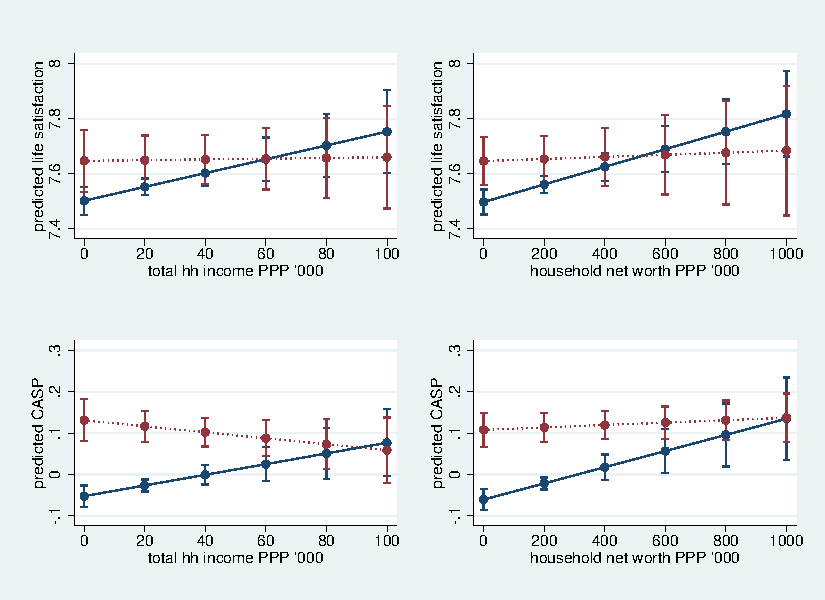
\includegraphics[width=4in]{/tmp/shareElderly/regDmarg.pdf}  
  \caption{SWB  (life satisfaction and CASP) against income, wealth, and
    pensions for volunteers (dotted line) and non-volunteers (solid line).}
  \label{mar}
\end{figure}


% or take scanario of middle class family with ??? v rich family ???: for the midlle
% class the rlationship betwene volnteering and swb is about 2x
%there are some such results in dofile



Interestingly,  the
relationship with pension is flat or even opposite to that of income or wealth--the higher the
pension, the stronger the effect from volunteering.\footnote{Still, results are
statistically insignificant for life satisfaction and only significant for CASP.} One explanation is that
pensions do not require time (as opposed to labor income), and provide peace of
mind and let one engage in volunteering as opposed to paid labor. 

With income and household net worth: clearly there is an opportunity cost. The rich could give to charity couple
millions, rather than help the kids cross the street. People give what they
have--rich have money, poor have time.  Note that prosocial spending also
contributes to SWB \citep{aknin13}.
%
With pensions the relationship is flat because there is no opportunity cost--you
get what you get.

%LATER wonder if if opportunity cost if inteacted with other social activities
%index! index of all activiies.  


Likewise, results in table \ref{regEw6} show that elders
who are retired derive more wellbeing from volunteering. This makes sense--they
have more time and lower opportunity cost. 
%

\begin{spacing}{.9}
\begin{table}[H]\centering \caption{OLS of SWB  (life satisfaction and CASP) on
    volunteering and pensions.  Unstandardized coefficients reported. All models
  include country dummies.}  \begin{scriptsize} \begin{tabular}{p{1.8in}p{.5in}p{.5in}p{.5in}p{.5in}|p{.5in}p{.5in}p{.5in}p{.5in}p{.5in}p{.4in}p{.5in}p{.4in}}\hline &\multicolumn{4}{c}{Life satisfaction}&\multicolumn{4}{c}{CASP}\\
                    &          e1   &          e2   &          e3   &          e4   &          e5   &          e6   &          e7   &          e8   \\
no voluneering/charity&      0.0000   &      0.0000   &      0.0000   &      0.0000   &      0.0000   &      0.0000   &      0.0000   &      0.0000   \\
voluneering/charity &      0.4611***&      0.1433** &      0.3380***&      0.0629   &      0.4497***&      0.1860***&      0.3544***&      0.1140***\\
employed=0          &      0.0000   &      0.0000   &               &               &               &               &               &               \\
employed=1          &      0.2869***&      0.1681***&               &               &               &               &               &               \\
no voluneering/charity $\times$ employed=0&      0.0000   &      0.0000   &               &               &               &               &               &               \\
no voluneering/charity $\times$ employed=1&      0.0000   &      0.0000   &               &               &               &               &               &               \\
voluneering/charity $\times$ employed=0&      0.0000   &      0.0000   &               &               &               &               &               &               \\
voluneering/charity $\times$ employed=1&     -0.2571** &     -0.1472+  &               &               &               &               &               &               \\
employed            &               &               &               &      0.1460** &      0.4270***&      0.0000   &               &      0.0894***\\
total hh income PPP '000&               &      0.0023** &               &      0.0028***&               &               &               &      0.0009*  \\
Total household expenditure PPP '000&               &      0.0030   &               &      0.0021   &               &      0.0078***&               &      0.0066***\\
household net worth PPP '000&               &      0.0003***&               &               &               &      0.0002***&               &               \\
attended an educational or training course&               &      0.0432   &               &      0.0446   &               &      0.0567** &               &      0.0548** \\
gone to a sport, social or other kind of club&               &      0.1619***&               &      0.1711***&               &      0.1284***&               &      0.1326***\\
taken part in a political or community-related organization&               &     -0.0081   &               &     -0.0050   &               &      0.0534*  &               &      0.0535*  \\
read books, magazines or newspapers&               &      0.2992***&               &      0.3075***&               &      0.2162***&               &      0.2201***\\
did word or number games (crossword puzzles/Sudoku...)&               &      0.0664*  &               &      0.0649+  &               &      0.0787***&               &      0.0769***\\
played cards or games such as chess&               &      0.1018** &               &      0.1013** &               &      0.0585***&               &      0.0576***\\
male                &               &      0.0289   &               &      0.0286   &               &      0.0783***&               &      0.0732***\\
married and living together&               &      0.5362***&               &      0.5511***&               &      0.1677***&               &      0.1744***\\
age                 &               &      0.0265***&               &      0.0269***&               &      0.0003   &               &      0.0000   \\
years of education  &               &      0.0020   &               &      0.0038   &               &      0.0073***&               &      0.0079***\\
number of children  &               &      0.0122   &               &      0.0115   &               &     -0.0088   &               &     -0.0090   \\
self reported health&               &      0.5470***&               &      0.5528***&               &      0.3595***&               &      0.3625***\\
pension             &               &               &      0.0000** &     -0.0000   &               &               &      0.0000   &      0.0000   \\
no voluneering/charity $\times$ pension&               &               &      0.0000   &      0.0000   &               &               &      0.0000   &      0.0000   \\
voluneering/charity $\times$ pension&               &               &      0.0000   &      0.0000   &               &               &      0.0000   &      0.0000+  \\
no voluneering/charity $\times$ employed&               &               &               &               &      0.0000   &      0.0000   &               &               \\
voluneering/charity $\times$ employed&               &               &               &               &     -0.2543***&     -0.1320***&               &               \\
country dummies&yes&yes&yes&yes&yes&yes&yes&yes\\
constant            &      8.0711***&      3.8225***&      8.1191***&      3.8005***&      0.1479***&     -1.4125***&      0.2886***&     -1.3963***\\
N                   &       62967   &       62967   &       62967   &       62967   &       61492   &       61492   &       61492   &       61492   \\

      \hline\multicolumn{5}{l}{+p$<$0.10 *p$<$0.05 **p$<$0.01 ***p$<$0.001,
        robust std err} \end{tabular}\label{regEw6} \end{scriptsize}\end{table}
\end{spacing}





\section*{Conclusion and discussion}

We found support for $H_1:$ The more social transfers and social capital,
especially in the form of volunteering, the more SWB.
This study adds another piece of evidence to a line of research arguing that
volunteering is a productive aging strategy
\citep[e.g.,][]{wilson12B,hank09}--here productive means increasing SWB.
It is especially important given that the burden of aging %hank05 used the term
 is increasing--all European countries are aging--and younger generations will
 have to increasingly pay more for the elderly. It is important to highlight that elderly have greater potential to volunteer as
they have more time, especially the elderly who are retired. But even those in
paid labor, arguably tend to have less harried schedule than younger workers.
% : those that are active live longer and better; if you
% do nothing you die qucik


We also found support for $H_2:$ When considered simultaneously pensions and volunteering have about the same effect on SWB.
Yet, volunteering (or anything else for that matter) cannot be a complete alternative
or a substitute to social transfers--one needs to be able to afford necessities.
But it can be a significant complement and it can tradeoff some of the decrease in transfers.

There is a related issue of retirement age--while people live longer, it is
 politically difficult to increase retirement age--but this is not economically
 sustainable. Volunteering can help--for instance, people can still be retiring
 earlier but if they remain productive through volunteering they can generate
 free products and services, which would ease budget expenditures and help with
 deficits. Indeed, in spirit of nudging as opposed to forcing people
 \citep{thaler08}, we suggest such policy: increase retirement age, but allow a
 person to retire early if she volunteers.\footnote{The devil is in the details
   of course--it remains to be worked out how to exactly design and implement
   such policy.}

Europe is aging: Fewer babies are born, and Europeans live longer, and healthcare
costs are increasing. So people live longer and in better shape, and at the same
time retirement age increase is opposed, so there are more untapped resources in
terms of labor that elderly could perform. We suggest volunteering--especially
in countries with low levels of volunteering, there is a great deal of
potential.\footnote{Our preliminary results (not shown here) suggest that the
  effect of volunteering on SWB has strongest potential for growth among
  countries with low levels of volunteering.}  
%
%
 For instance, in western countries many public utility tasks are performed by volunteers such
as helping kids cross the street. In east, on the other hand, these activities
are often performed by paid labor that could be used better elsewhere, for
instance, in Poland % Straz Miejska
 city employees often helps kids cross the street. %leszek morawski per ozarow
 In the US, it is often volunteers.

In this study we focused on overall patterns (controlling for country level fixed
effects). Future research can explore differences across countries. 
%
The goal of this study was to focus on the general relationships and the tradeoff
between economic and social capitals.

SHARE are very rich data and there can be much more done in terms of narrowing
down and measuring pensions and volunteering. And related concepts can be
measured, too. For instance, we have found that volunteering works better for
poorer persons and suggested that for richer persons giving may contribute more
to their SWB. This can be tested using FT001, FT002, FT003, and other FT
variables.  



Future research could look at effect of earlier life experiences effect on successful
aging. For instance, \citet{pruchno2010successful,pruchno2010two} found in the US that incarceration,
 marital, work, and volunteer statuses, as well as moderate
alcohol consumption affect successful aging--such approach could be
replicated in Europe using SHARELIFE, SHARE's module focused on people's life
histories. In particular, it would be interesting to examine effect of earlier
volunteering in life on successful aging later--perhaps, not only
volunteering later in life, but also earlier has a positive effect. 

As any correlational study, causality cannot be established. While panel data
does not help much with causality,  (an experiment or natural experiment is
needed), panel data does help controlling for unobservable heterogeneity if it is
time constant. 

We did not test for actual substitution, ie take away one (social  capital) and replace
with another one (economic capital) and SWB remains constant--our results
suggest that indeed it may be the case (at least to some degree; again, one
needs at least some economic capital that cannot be easily replaced with other
capitals). It is a great topic for future research.

To advance policy making and
administration we should ask how much happiness will a policy bring
about. There are always limited resources, and there are many competing needs: education, safety, public
health, and so forth. One metric to help direct spending is SWB.\footnote{Of
  course, it is not the only metric, neither a perfect one. There are other
  considerations--notably not everything that makes us happy is the right thing
  to do. However, if an activity (e.g., volunteering) has other benefits and few if any
  disadvantages, then SWB yardstick is more appropriate.}
Key  advantage of happiness yardstick is that it overcomes difficulty
of measuring utility in social welfare, for instance, it helps to answer
a question whether we should  invest
limited resources in pensions, healthcare, or infrastructure.
% You don't have to be a utilitarian to agree that a major goal of
% public policy making is achieving ``the greatest happiness for the greatest
% number.'' 

%--------------------

Neighborhood support groups have always played a key role in helping the poor
survive \citep{saegert2002social}, and so do individual persons play a key role
helping other poor \citep{mazelis2017surviving}. Most countries experience
rising inequality \citep{piketty03,mackintosh13,oecd08,verbeek15}--the middle
class is diminishing\footnote{For the world as a whole, the inequality is
  decreasing due to the poor countries, notably China, catching up--in many poor
  countries, middle class is actually increasing.}, and it is becoming two classes: the rich and the
rest. Our results suggest that volunteering may not be the viable strategy for the rich, but it is for the rest.
 




% %table centered on decimal points:)
% \begin{table}[H]\centering\footnotesize
% \caption{\label{freq_im_god} importance of God}
% \begin{tabular} {@{} lrrrr @{}}   \hline 
% Item& Number & Per cent   \\ \hline
% 1(not at all)&    9,285&  9\\
% 2&    3,555&        3\\
% 3&    3,937&        4\\
% 4&    2,888&        3\\
% 5&    7,519&        7\\
% 6&    5,175&        5\\
% 7&    6,050&        6\\
% 8&    8,067&        8\\
% 9&    8,463&        8\\
% 10&   52,385&       49\\
% Total&  107,324&      100\\ \hline
% \end{tabular}\end{table}


% % Define block styles
% \tikzstyle{block} = [rectangle, draw, fill=black!20, 
%     text width=10em, text centered, rounded corners, minimum height=4em]
% \tikzstyle{b} = [rectangle, draw,  
%     text width=6em, text centered, rounded corners, minimum height=4em]
% \tikzstyle{line} = [draw, -latex']
% \tikzstyle{cloud} = [draw, ellipse,fill=black!20, node distance = 5cm,
%     minimum height=2em]
    
% \begin{tikzpicture}[node distance = 2cm, auto]
%     % Place nodes
%     \node [block] (lib) {liberalism, egalitarianism, welfare};
%     \node [block, below of=lib] (con) {conservatism, competition, individualism};
%     \node [cloud, right of=con] (ls) {well-being};
%     \node [block, below of=ls] (cul) {genes, culture};
%     \node [b, left of =lib, node distance = 4cm] (c) {country-level};
%     \node [b, left of =con,  node distance = 4cm] (c) {person-level};
%     % Draw edges
%     \path [line] (lib) -- (ls);
%     \path [line] (con) -- (ls);
%     \path [line,dashed] (cul) -- (ls);
% \end{tikzpicture}


%PUT THIS NOTE, polish and put to /root/author_what_data --ALWAYS
%stick here stuff as i run it!!! maybe comment out later...

% \section*{\Huge ONLINE APPENIX}
% \textbf{[note: this section will NOT be a part of the final version of
%   the manuscript, but will be available online instead]} %hence everything below
%                                 %is organized byu section, not subsection
% !!!
% have most of the stuff outputted to online appendix:)--start with that and then
% select stuff to paper--have brief narrative describng patterns in online app too
% !!!

% \section*{Variables' definitions, coding, and distributions}
% \label{app_var_des}


% %\input{/tmp/a.tex} %aok_var_des

% % \begin{spacing}{.9}
% %   \begin{table}[H]\centering \caption{Summary statistics.} \label{sumSta} \begin{scriptsize} \begin{tabular}{p{1.8in}p{.5in}p{.5in}p{.5in}p{.5in}p{.5in}p{.5in}p{.5in}p{.5in}p{.5in}p{.5
% %             in}p{.5in}p{.5 in}}\hline
% %         \input{/tmp/aha2.tex}
% %          \end{tabular}\end{scriptsize}\end{table}
% % \end{spacing}

% % \begin{spacing}{.9}
% %   \begin{table}[H]\centering \caption{Correlation matrix.} \label{sumSta} \begin{scriptsize} \begin{tabular}{@{}
% %           p{1.2in} rrrrrrrrrrrrr @{}}\hline
% %         \input{/tmp/ahb2.tex}\hline
% %          \end{tabular}\end{scriptsize}\end{table}
% % \end{spacing}



% Table XXX shows variable distributions. If a variable has more than
% 10 categories it is classified into bins...

% %\input .... %TODO !!!! have input here histograms

% \section*{Additional Descriptive Statistics}
% \label{app_des_sta}

% %make sure i have [H] or h! ???
% % \begin{table}[H]
% % \caption{}
% % \centering
% % \label{}
% % \begin{scriptsize}
% % \input{../out/reg_c.tex}
% % \end{scriptsize}
% % \end{table}

%\newpage
%\theendnotes
%\bibliography{/home/aok/papers/root/tex/ebib.bib,socTraSocCap.bib}

\begin{thebibliography}{87}
\newcommand{\enquote}[1]{``#1''}
\expandafter\ifx\csname natexlab\endcsname\relax\def\natexlab#1{#1}\fi

\bibitem[\protect\citeauthoryear{Aknin, Barrington-Leigh, Dunn, Helliwell,
  Burns, Biswas-Diener, Kemeza, Nyende, Ashton-James, and Norton}{Aknin
  et~al.}{2013}]{aknin13}
\textsc{Aknin, L.~B., C.~P. Barrington-Leigh, E.~W. Dunn, J.~F. Helliwell,
  J.~Burns, R.~Biswas-Diener, I.~Kemeza, P.~Nyende, C.~E. Ashton-James, and
  M.~I. Norton} (2013): \enquote{Prosocial spending and well-being:
  Cross-cultural evidence for a psychological universal.} \emph{Journal of
  Personality and Social Psychology}, 104, 635.

\bibitem[\protect\citeauthoryear{Alesina, Glaeser, and Sacerdote}{Alesina
  et~al.}{2001}]{alesina01}
\textsc{Alesina, A., E.~L. Glaeser, and B.~Sacerdote} (2001): \enquote{Why
  Doesn't the United States Have a European-Style Welfare State,}
  \emph{Brookings Papers on Economic Activity}, 187--254.

\bibitem[\protect\citeauthoryear{Alesina, Glaeser, and Sacerdote}{Alesina
  et~al.}{2005}]{alesina05al}
---\hspace{-.1pt}---\hspace{-.1pt}--- (2005): \enquote{Work and Leisure in the
  U.S. and Europe: Why So Different?} Working Paper 278, National Bureau of
  Economic Research.

\bibitem[\protect\citeauthoryear{Alvarez-Diaz, Gonzalez, and
  Radcliff}{Alvarez-Diaz et~al.}{2009}]{alvarez09}
\textsc{Alvarez-Diaz, A., L.~Gonzalez, and B.~Radcliff} (2009): \enquote{{The
  politics of happiness: On the political determinants of quality of life in
  the American States},} \emph{Unpublished Manuscript}.

\bibitem[\protect\citeauthoryear{Amit and Litwin}{Amit and
  Litwin}{2010}]{amit2010subjective}
\textsc{Amit, K. and H.~Litwin} (2010): \enquote{The subjective well-being of
  immigrants aged 50 and older in Israel,} \emph{Social indicators research},
  98, 89--104.

\bibitem[\protect\citeauthoryear{Anderson, Damianakis, Kr{\"o}ger, Wagner,
  Dawson, Binns, Bernstein, Caspi, and Cook}{Anderson
  et~al.}{2014}]{anderson14}
\textsc{Anderson, N.~D., T.~Damianakis, E.~Kr{\"o}ger, L.~M. Wagner, D.~R.
  Dawson, M.~A. Binns, S.~Bernstein, E.~Caspi, and S.~L. Cook} (2014):
  \enquote{The benefits associated with volunteering among seniors: a critical
  review and recommendations for future research.} \emph{Psychological
  bulletin}, 140, 1505.

\bibitem[\protect\citeauthoryear{Angelini, Cavapozzi, Corazzini, and
  Paccagnella}{Angelini et~al.}{2012}]{angelini2012age}
\textsc{Angelini, V., D.~Cavapozzi, L.~Corazzini, and O.~Paccagnella} (2012):
  \enquote{Age, health and life satisfaction among older Europeans,}
  \emph{Social indicators research}, 105, 293--308.

\bibitem[\protect\citeauthoryear{Ashkanasy}{Ashkanasy}{2011}]{ashkanasy11}
\textsc{Ashkanasy, N.~M.} (2011): \enquote{International Happiness: A
  Multilevel Perspective,} \emph{The Academy of Management Perspectives}, 25,
  23--29.

\bibitem[\protect\citeauthoryear{Bender}{Bender}{2012}]{bender12}
\textsc{Bender, K.~A.} (2012): \enquote{An analysis of well-being in
  retirement: The role of pensions, health, of retirement,} \emph{The Journal
  of Socio-Economics}, 41, 424--433.

\bibitem[\protect\citeauthoryear{Blanchflower and Oswald}{Blanchflower and
  Oswald}{2011}]{blanchflower11}
\textsc{Blanchflower, D.~G. and A.~J. Oswald} (2011): \enquote{International
  happiness: A new view on the measure of performance,} \emph{The Academy of
  Management Perspectives}, 25, 6--22.

\bibitem[\protect\citeauthoryear{Blom and Schr{\"o}der}{Blom and
  Schr{\"o}der}{2011}]{blom2011sample}
\textsc{Blom, A.~G. and M.~Schr{\"o}der} (2011): \enquote{Sample composition 4
  years on: retention in SHARE Wave 3,} \emph{Retrospective data collection in
  the Survey of Health, Ageing and Retirement in Europe}, 55--61.

\bibitem[\protect\citeauthoryear{Bok}{Bok}{2010}]{bok10}
\textsc{Bok, D.} (2010): \emph{The politics of happiness: What government can
  learn from the new research on well-being}, Princeton University Press,
  Princeton NJ.

\bibitem[\protect\citeauthoryear{Bonsang and van Soest}{Bonsang and van
  Soest}{2012}]{bonsang12}
\textsc{Bonsang, E. and A.~van Soest} (2012): \enquote{Satisfaction with social
  contacts of older Europeans,} \emph{Social indicators research}, 105,
  273--292.

\bibitem[\protect\citeauthoryear{Borgonovi}{Borgonovi}{2008}]{borgonovi2008doing}
\textsc{Borgonovi, F.} (2008): \enquote{Doing well by doing good. The
  relationship between formal volunteering and self-reported health and
  happiness,} \emph{Social science \& medicine}, 66, 2321--2334.

\bibitem[\protect\citeauthoryear{Butrica and Schaner}{Butrica and
  Schaner}{2005}]{butrica2005satisfaction}
\textsc{Butrica, B.~A. and S.~G. Schaner} (2005): \enquote{Satisfaction and
  engagement in retirement,} .

\bibitem[\protect\citeauthoryear{Campbell, Converse, and Rodgers}{Campbell
  et~al.}{1976}]{campbell76etal}
\textsc{Campbell, A., P.~E. Converse, and W.~L. Rodgers} (1976): \emph{The
  quality of American life: perceptions, evaluations, and satisfactions},
  Russell Sage Foundation, New York NY.

\bibitem[\protect\citeauthoryear{De~Tocqueville}{De~Tocqueville}{2003}]{tocqueville03}
\textsc{De~Tocqueville, A.} (2003): \emph{Democracy in America}, vol.~10,
  Gateway Editions.

\bibitem[\protect\citeauthoryear{{Di Tella} and MacCulloch}{{Di Tella} and
  MacCulloch}{2006}]{ditella06m}
\textsc{{Di Tella}, R. and R.~MacCulloch} (2006): \enquote{Some Uses of
  Happiness Data in Economics,} \emph{The Journal of Economic Perspectives},
  20, 25--46.

\bibitem[\protect\citeauthoryear{{Di Tella}, MacCulloch, and Oswald}{{Di Tella}
  et~al.}{2001{\natexlab{a}}}]{ditella01mob}
\textsc{{Di Tella}, R., R.~J. MacCulloch, and A.~J. Oswald}
  (2001{\natexlab{a}}): \enquote{The macroeconomics of happiness,} Warwick
  Economic Research Papers No 615.

\bibitem[\protect\citeauthoryear{{Di Tella}, MacCulloch, and Oswald}{{Di Tella}
  et~al.}{2001{\natexlab{b}}}]{ditella01moa}
---\hspace{-.1pt}---\hspace{-.1pt}--- (2001{\natexlab{b}}):
  \enquote{Preferences over inflation and unemployment: Evidence from surveys
  of happiness,} \emph{American Economic Review}, 91, 335--341.

\bibitem[\protect\citeauthoryear{Diener}{Diener}{2009}]{diener09}
\textsc{Diener, E.} (2009): \emph{Well-being for public policy}, Oxford
  University Press, New York NY.

\bibitem[\protect\citeauthoryear{Diener and Seligman}{Diener and
  Seligman}{2004}]{diener04s}
\textsc{Diener, E. and M.~E.~P. Seligman} (2004): \enquote{Beyond Money: Toward
  an Economy of Well-being,} \emph{Psychological Science}, 5, 1--31.

\bibitem[\protect\citeauthoryear{Dingemans and Henkens}{Dingemans and
  Henkens}{2014}]{dingemans2014involuntary}
\textsc{Dingemans, E. and K.~Henkens} (2014): \enquote{Involuntary retirement,
  bridge employment, and satisfaction with life: A longitudinal investigation,}
  \emph{Journal of Organizational Behavior}, 35, 575--591.

\bibitem[\protect\citeauthoryear{Dingemans and Henkens}{Dingemans and
  Henkens}{2015}]{dingemans2015retirement}
---\hspace{-.1pt}---\hspace{-.1pt}--- (2015): \enquote{How do retirement
  dynamics influence mental well-being in later life? A 10-year panel study,}
  \emph{Scand J Work Environ Health}, 41, 16--23.

\bibitem[\protect\citeauthoryear{Dolan, Peasgood, and White}{Dolan
  et~al.}{2008}]{dolan08al}
\textsc{Dolan, P., T.~Peasgood, and M.~White} (2008): \enquote{Do We Really
  Know What Makes Us Happy A Review of the Economic Literature on the Factors
  Associated with Subjective Well-being,} \emph{Journal of Economic
  Psychology}, 29, 94--122.

\bibitem[\protect\citeauthoryear{Dulin, Gavala, Stephens, Kostick, and
  McDonald}{Dulin et~al.}{2012}]{dulin2012volunteering}
\textsc{Dulin, P.~L., J.~Gavala, C.~Stephens, M.~Kostick, and J.~McDonald}
  (2012): \enquote{Volunteering predicts happiness among older M{\=a}ori and
  non-M{\=a}ori in the New Zealand health, work, and retirement longitudinal
  study,} \emph{Aging \& mental health}, 16, 617--624.

\bibitem[\protect\citeauthoryear{Easterlin, McVey, Switek, Sawangfa, and
  Zweig}{Easterlin et~al.}{2010}]{easterlin10B}
\textsc{Easterlin, R.~A., L.~A. McVey, M.~Switek, O.~Sawangfa, and J.~S. Zweig}
  (2010): \enquote{The happiness--income paradox revisited,} \emph{Proceedings
  of the National Academy of Sciences}, 107, 22463--22468.

\bibitem[\protect\citeauthoryear{{Ferrer-i-Carbonell} and
  Frijters}{{Ferrer-i-Carbonell} and Frijters}{2004}]{carbonell04}
\textsc{{Ferrer-i-Carbonell}, A. and P.~Frijters} (2004): \enquote{How
  Important is Methodology for the Estimates of the Determinants of Happiness?}
  \emph{Economic Journal}, 114, 641--659.

\bibitem[\protect\citeauthoryear{Ferring and Boll}{Ferring and
  Boll}{2010}]{ferring10}
\textsc{Ferring, D. and T.~Boll} (2010): \enquote{Subjective wellbeing in older
  adults: Current state and gaps of research,} in \emph{Ageing, health and
  pensions in Europe}, ed. by A.~Z. Lans~Bovenberg, Arthur van~Soest, Springer,
  173--212.

\bibitem[\protect\citeauthoryear{Fischer}{Fischer}{2010}]{fischer10}
\textsc{Fischer, C.~S.} (2010): \emph{Made in America: A social history of
  American culture and character}, University of Chicago Press, Chicago IL.

\bibitem[\protect\citeauthoryear{Frijters, Haisken-Denew, and Shields}{Frijters
  et~al.}{2004}]{frijters04}
\textsc{Frijters, P., J.~P. Haisken-Denew, and M.~a. Shields} (2004):
  \enquote{{Money does matter! evidence from increasing real income and life
  satisfaction in east germany following reunification},} \emph{American
  Economic Review}, 94, 730--740.

\bibitem[\protect\citeauthoryear{Gwozdz and Sousa-Poza}{Gwozdz and
  Sousa-Poza}{2010}]{gwozdz10}
\textsc{Gwozdz, W. and A.~Sousa-Poza} (2010): \enquote{Ageing, health and life
  satisfaction of the oldest old: An analysis for Germany,} \emph{Social
  Indicators Research}, 97, 397--417.

\bibitem[\protect\citeauthoryear{Hank and Erlinghagen}{Hank and
  Erlinghagen}{2009}]{hank09}
\textsc{Hank, K. and M.~Erlinghagen} (2009): \enquote{Dynamics of volunteering
  in older Europeans,} \emph{The Gerontologist}, 50, 170--178.

\bibitem[\protect\citeauthoryear{Haski-Leventhal}{Haski-Leventhal}{2009}]{haski09}
\textsc{Haski-Leventhal, D.} (2009): \enquote{Elderly volunteering and
  well-being: A cross-European comparison based on SHARE data,} \emph{Voluntas:
  International Journal of Voluntary and Nonprofit Organizations}, 20,
  388--404.

\bibitem[\protect\citeauthoryear{Hyde, Higgs, Wiggins, and Blane}{Hyde
  et~al.}{2015}]{hyde15}
\textsc{Hyde, M., P.~Higgs, R.~Wiggins, and D.~Blane} (2015): \enquote{A decade
  of research using the CASP scale: key findings and future directions,} .

\bibitem[\protect\citeauthoryear{Hyde, Wiggins, Higgs, and Blane}{Hyde
  et~al.}{2003{\natexlab{a}}}]{hyde03}
\textsc{Hyde, M., R.~D. Wiggins, P.~Higgs, and D.~B. Blane}
  (2003{\natexlab{a}}): \enquote{A measure of quality of life in early old age:
  the theory, development and properties of a needs satisfaction model
  (CASP-19),} \emph{Aging \& mental health}, 7, 186--194.

\bibitem[\protect\citeauthoryear{Hyde, Wiggins, Higgs, and Blane}{Hyde
  et~al.}{2003{\natexlab{b}}}]{hyde2003measure}
---\hspace{-.1pt}---\hspace{-.1pt}--- (2003{\natexlab{b}}): \enquote{A measure
  of quality of life in early old age: the theory, development and properties
  of a needs satisfaction model (CASP-19),} \emph{Aging \& mental health}, 7,
  186--194.

\bibitem[\protect\citeauthoryear{Jenkinson, Dickens, Jones, Thompson-Coon,
  Taylor, Rogers, Bambra, Lang, and Richards}{Jenkinson
  et~al.}{2013}]{jenkinson2013volunteering}
\textsc{Jenkinson, C.~E., A.~P. Dickens, K.~Jones, J.~Thompson-Coon, R.~S.
  Taylor, M.~Rogers, C.~L. Bambra, I.~Lang, and S.~H. Richards} (2013):
  \enquote{Is volunteering a public health intervention? A systematic review
  and meta-analysis of the health and survival of volunteers,} \emph{BMC public
  health}, 13, 773.

\bibitem[\protect\citeauthoryear{J{\"u}rges and van Soest}{J{\"u}rges and van
  Soest}{2012}]{jurges12}
\textsc{J{\"u}rges, H. and A.~van Soest} (2012): \enquote{Comparing the
  well-being of older europeans: Introduction,} \emph{Social indicators
  research}, 105, 187--190.

\bibitem[\protect\citeauthoryear{Kahneman and Deaton}{Kahneman and
  Deaton}{2010}]{kahneman10}
\textsc{Kahneman, D. and A.~Deaton} (2010): \enquote{High income improves
  evaluation of life but not emotional well-being,} \emph{Proceedings of the
  National Academy of Sciences}, 107, 16489--16493.

\bibitem[\protect\citeauthoryear{Kahneman, Diener, and Schwarz}{Kahneman
  et~al.}{1999}]{kahneman99}
\textsc{Kahneman, D., E.~Diener, and N.~Schwarz} (1999): \emph{Well-being:
  Foundations of hedonic psychology}, Russell Sage Foundation.

\bibitem[\protect\citeauthoryear{Kim, Netuveli, Blane, Peasey, Malyutina,
  Simonova, Kubinova, Pajak, Croezen, Bobak et~al.}{Kim
  et~al.}{2015}]{kim2015psychometric}
\textsc{Kim, G.~R., G.~Netuveli, D.~Blane, A.~Peasey, S.~Malyutina,
  G.~Simonova, R.~Kubinova, A.~Pajak, S.~Croezen, M.~Bobak, et~al.} (2015):
  \enquote{Psychometric properties and confirmatory factor analysis of the
  CASP-19, a measure of quality of life in early old age: the HAPIEE study,}
  \emph{Aging \& mental health}, 19, 595--609.

\bibitem[\protect\citeauthoryear{Klein and Kozlowski}{Klein and
  Kozlowski}{2000}]{klein00}
\textsc{Klein, K.~J. and S.~W. Kozlowski} (2000): \enquote{From micro to meso:
  Critical steps in conceptualizing and conducting multilevel research,}
  \emph{Organizational Research Methods}, 3, 211--236.

\bibitem[\protect\citeauthoryear{Knesbeck, Hyde, Higgs, Kurlan, and
  Siegrist}{Knesbeck et~al.}{2005}]{knesbeck2005quality}
\textsc{Knesbeck, O., M.~Hyde, P.~Higgs, R.~Kurlan, and J.~Siegrist} (2005):
  \enquote{Quality of life and well-being,} .

\bibitem[\protect\citeauthoryear{Kushlev, Dunn, and Lucas}{Kushlev
  et~al.}{2015}]{kushlev15}
\textsc{Kushlev, K., E.~W. Dunn, and R.~E. Lucas} (2015): \enquote{Higher
  Income Is Associated With Less Daily Sadness but not More Daily Happiness,}
  \emph{Social Psychological and Personality Science}, 6, 483--489.

\bibitem[\protect\citeauthoryear{Layard}{Layard}{2005}]{layard05}
\textsc{Layard, R.} (2005): \emph{Happiness. Lessons from a new science.}, The
  Penguin Press, New York NY.

\bibitem[\protect\citeauthoryear{Lipset and Marks}{Lipset and
  Marks}{2000}]{lipset00}
\textsc{Lipset, S.~M. and G.~Marks} (2000): \emph{It didn't happen here: why
  socialism failed in the United States}, WW Norton \& Company, New York NY.

\bibitem[\protect\citeauthoryear{Luttmer}{Luttmer}{2005}]{luttmer05}
\textsc{Luttmer, E. F.~P.} (2005): \enquote{Neighbors as Negatives: Relative
  Earnings and Well-Being,} \emph{Quarterly Journal of Economics}, 120,
  963--02.

\bibitem[\protect\citeauthoryear{Mackintosh}{Mackintosh}{2013}]{mackintosh13}
\textsc{Mackintosh, E.} (2013): \enquote{Report: Income Inequality Rising in
  Most Developed Countries,} \emph{Washington Post}.

\bibitem[\protect\citeauthoryear{Maslow}{Maslow}{[1954] 1987}]{maslow87}
\textsc{Maslow, A.} ([1954] 1987): \emph{{Motivation and personality}},
  Longman, 3 ed.

\bibitem[\protect\citeauthoryear{Mazelis}{Mazelis}{2017}]{mazelis2017surviving}
\textsc{Mazelis, J.~M.} (2017): \emph{Surviving Poverty: Creating Sustainable
  Ties Among the Poor}, NYU Press.

\bibitem[\protect\citeauthoryear{Meier and Stutzer}{Meier and
  Stutzer}{2008{\natexlab{a}}}]{meier2008volunteering}
\textsc{Meier, S. and A.~Stutzer} (2008{\natexlab{a}}): \enquote{Is
  volunteering rewarding in itself?} \emph{Economica}, 75, 39--59.

\bibitem[\protect\citeauthoryear{Meier and Stutzer}{Meier and
  Stutzer}{2008{\natexlab{b}}}]{meier08}
---\hspace{-.1pt}---\hspace{-.1pt}--- (2008{\natexlab{b}}): \enquote{Is
  volunteering rewarding in itself?} \emph{Economica}, 75, 39--59.

\bibitem[\protect\citeauthoryear{Michalos}{Michalos}{1985}]{michalos85}
\textsc{Michalos, A.} (1985): \enquote{Multiple discrepancies theory (MDT),}
  \emph{Social Indicators Research}, 16, 347--413.

\bibitem[\protect\citeauthoryear{Mujcic and Oswald}{Mujcic and
  Oswald}{2017}]{mujcic17}
\textsc{Mujcic, R. and A.~J. Oswald} (2017): \enquote{Is envy harmful to a
  society's psychological health and wellbeing? A longitudinal study of 18,000
  adults,} \emph{Social Science \& Medicine}.

\bibitem[\protect\citeauthoryear{Myers}{Myers}{2000}]{myers00}
\textsc{Myers, D.~G.} (2000): \enquote{The Funds, Friends, and Faith of Happy
  People,} \emph{American Psychologist}, 55, 56--67.

\bibitem[\protect\citeauthoryear{Nikolova and Graham}{Nikolova and
  Graham}{2014}]{nikolova2014employment}
\textsc{Nikolova, M. and C.~Graham} (2014): \enquote{Employment, late-life
  work, retirement, and well-being in Europe and the United States,} \emph{IZA
  Journal of European Labor Studies}, 3, 1--30.

\bibitem[\protect\citeauthoryear{OECD}{OECD}{2008}]{oecd08}
\textsc{OECD} (2008): \enquote{Income inequality and poverty rising in most
  OECD countries,} \emph{OECD Press Release:
  \url{http://www.oecd.org/general/incomeinequalityandpovertyrisinginmostoecdcountries.htm}}.

\bibitem[\protect\citeauthoryear{Okulicz-Kozaryn}{Okulicz-Kozaryn}{2013}]{aok13liavbility}
\textsc{Okulicz-Kozaryn, A.} (2013): \enquote{City Life: Rankings (Livability)
  Versus Perceptions (Satisfaction),} \emph{Social Indicators Research}, 110,
  433--451.

\bibitem[\protect\citeauthoryear{Okulicz-Kozaryn}{Okulicz-Kozaryn}{2016}]{aok_lsPol16}
---\hspace{-.1pt}---\hspace{-.1pt}--- (2016): \enquote{Happiness Research for
  Public Policy and Administration,} \emph{Transforming Government: People,
  Process and Policy}.

\bibitem[\protect\citeauthoryear{Okulicz-Kozaryn, Holmes~IV, and
  Avery}{Okulicz-Kozaryn et~al.}{2014}]{aokJap14}
\textsc{Okulicz-Kozaryn, A., O.~Holmes~IV, and D.~R. Avery} (2014):
  \enquote{The Subjective Well-Being Political Paradox: Happy Welfare States
  and Unhappy Liberals.} \emph{Journal of Applied Psychology}, 99, 1300--1308.

\bibitem[\protect\citeauthoryear{Okulicz-Kozaryn and Mazelis}{Okulicz-Kozaryn
  and Mazelis}{2016}]{aok_ruut_inc_ine}
\textsc{Okulicz-Kozaryn, A. and J.~M. Mazelis} (2016): \enquote{More Unequal In
  Income, More Unequal in Wellbeing,} \emph{Social Indicators Research}.

\bibitem[\protect\citeauthoryear{Okulicz-Kozaryn and Valente}{Okulicz-Kozaryn
  and Valente}{2018}]{aok-swbLivability18}
\textsc{Okulicz-Kozaryn, A. and R.~Valente} (2018): \enquote{Livability and
  Subjective Wellbeing Across European Cities,} \emph{Forthcoming in Applied
  Research in Quality of Life}.

\bibitem[\protect\citeauthoryear{Oswald}{Oswald}{2014}]{oswald14}
\textsc{Oswald, A.} (2014): \enquote{Keynote II,} \emph{2014 Wellbeing and
  Public Policy Conference at Hamilton College}.

\bibitem[\protect\citeauthoryear{Pacek and Radcliff}{Pacek and
  Radcliff}{2008{\natexlab{a}}}]{pacek08b}
\textsc{Pacek, A. and B.~Radcliff} (2008{\natexlab{a}}): \enquote{Assessing the
  welfare state: The politics of happiness,} \emph{Perspectives on Politics},
  6, 267--277.

\bibitem[\protect\citeauthoryear{Pacek and Radcliff}{Pacek and
  Radcliff}{2008{\natexlab{b}}}]{pacek08r}
---\hspace{-.1pt}---\hspace{-.1pt}--- (2008{\natexlab{b}}): \enquote{Welfare
  Policy and Subjective Well-Being Across Nations: An Individual-Level
  Assessment.} \emph{Social Indicators Research}, 89, 179 -- 191.

\bibitem[\protect\citeauthoryear{P{\'e}rez-Rojo, Mart{\'\i}n, Noriega, and
  L{\'o}pez}{P{\'e}rez-Rojo et~al.}{2017}]{perez2017psychometric}
\textsc{P{\'e}rez-Rojo, G., N.~Mart{\'\i}n, C.~Noriega, and J.~L{\'o}pez}
  (2017): \enquote{Psychometric properties of the CASP-12 in a Spanish older
  community dwelling sample,} \emph{Aging \& mental health}, 1--9.

\bibitem[\protect\citeauthoryear{Piketty and Saez}{Piketty and
  Saez}{2003}]{piketty03}
\textsc{Piketty, T. and E.~Saez} (2003): \enquote{Income inequality in the
  United States, 1913--1998,} \emph{The Quarterly Journal of Economics}, 118,
  1--41.

\bibitem[\protect\citeauthoryear{Pruchno, Wilson-Genderson, and
  Cartwright}{Pruchno et~al.}{2010{\natexlab{a}}}]{pruchno2010two}
\textsc{Pruchno, R.~A., M.~Wilson-Genderson, and F.~Cartwright}
  (2010{\natexlab{a}}): \enquote{A two-factor model of successful aging,}
  \emph{Journals of Gerontology Series B: Psychological Sciences and Social
  Sciences}, 65, 671--679.

\bibitem[\protect\citeauthoryear{Pruchno, Wilson-Genderson, Rose, and
  Cartwright}{Pruchno et~al.}{2010{\natexlab{b}}}]{pruchno2010successful}
\textsc{Pruchno, R.~A., M.~Wilson-Genderson, M.~Rose, and F.~Cartwright}
  (2010{\natexlab{b}}): \enquote{Successful aging: Early influences and
  contemporary characteristics,} \emph{The Gerontologist}, 50, 821--833.

\bibitem[\protect\citeauthoryear{Radcliff}{Radcliff}{2001}]{radcliff01}
\textsc{Radcliff, B.} (2001): \enquote{Politics, Markets, and Life
  Satisfaction: The Political Economy of Human Happiness,} \emph{American
  Political Science Review}, 95, 939--952.

\bibitem[\protect\citeauthoryear{Radcliff}{Radcliff}{2013}]{radcliff13}
---\hspace{-.1pt}---\hspace{-.1pt}--- (2013): \emph{The Political Economy of
  Human Happiness: How Voters' Choices Determine the Quality of Life},
  Cambridge University Press, New York NY.

\bibitem[\protect\citeauthoryear{Saegert, Thompson, and Warren}{Saegert
  et~al.}{2002}]{saegert2002social}
\textsc{Saegert, S., J.~P. Thompson, and M.~R. Warren} (2002): \emph{Social
  capital and poor communities}, Russell Sage Foundation.

\bibitem[\protect\citeauthoryear{Scruggs and Allan}{Scruggs and
  Allan}{2006}]{scruggs06Ba}
\textsc{Scruggs, L. and J.~Allan} (2006): \enquote{Welfare-state
  decommodification in 18 OECD countries: A replication and revision,}
  \emph{Journal of European Social Policy}, 16, 55--72.

\bibitem[\protect\citeauthoryear{Stolnitz}{Stolnitz}{1992}]{stolnitz1992demographic}
\textsc{Stolnitz, G.~J.} (1992): \enquote{Demographic causes and economic
  consequences of population aging: Europe and North America.} .

\bibitem[\protect\citeauthoryear{Thaler and Sunstein}{Thaler and
  Sunstein}{2008}]{thaler08}
\textsc{Thaler, R. and C.~Sunstein} (2008): \emph{Nudge: Improving decisions
  about health, wealth, and happiness}, Yale University Press.

\bibitem[\protect\citeauthoryear{Van~Willigen}{Van~Willigen}{2000}]{van2000differential}
\textsc{Van~Willigen, M.} (2000): \enquote{Differential benefits of
  volunteering across the life course,} \emph{The Journals of Gerontology
  Series B: Psychological Sciences and Social Sciences}, 55, S308--S318.

\bibitem[\protect\citeauthoryear{Vanhoutte}{Vanhoutte}{2012}]{vanhoutte12}
\textsc{Vanhoutte, B.} (2012): \enquote{Measuring subjective well-being: a
  review,} \emph{CCSR Woking Paper}.

\bibitem[\protect\citeauthoryear{Vanhoutte}{Vanhoutte}{2014}]{vanhoutte14}
---\hspace{-.1pt}---\hspace{-.1pt}--- (2014): \enquote{The multidimensional
  structure of subjective well-being in later life,} \emph{Journal of
  population ageing}, 7, 1--20.

\bibitem[\protect\citeauthoryear{Vaupel and Loichinger}{Vaupel and
  Loichinger}{2006}]{vaupel2006redistributing}
\textsc{Vaupel, J.~W. and E.~Loichinger} (2006): \enquote{Redistributing work
  in aging Europe,} \emph{Science}, 312, 1911--1913.

\bibitem[\protect\citeauthoryear{Veenhoven}{Veenhoven}{2008}]{veenhoven08}
\textsc{Veenhoven, R.} (2008): \enquote{Sociological theories of subjective
  well-being,} in \emph{The Science of Subjective Well-being: A tribute to Ed
  Diener}, ed. by M.~Eid and R.~Larsen, The Guilford Press, New York NY,
  44--61.

\bibitem[\protect\citeauthoryear{Veenhoven}{Veenhoven}{2012}]{veenhoven12}
---\hspace{-.1pt}---\hspace{-.1pt}--- (2012): \enquote{Evidence-based pursuit
  of happiness: What we should know, what we do know and what we can get to
  know,} Tech. rep., EHERO.

\bibitem[\protect\citeauthoryear{Verbeek}{Verbeek}{2015}]{verbeek15}
\textsc{Verbeek, J.} (2015): \enquote{Increasingly, inequality within, not
  across, countries is rising,} \emph{The World bank Development Talk
  \url{http://blogs.worldbank.org/developmenttalk/increasingly-inequality-within-not-across-countries-rising}}.

\bibitem[\protect\citeauthoryear{Wahrendorf, von~dem Knesebeck, and
  Siegrist}{Wahrendorf et~al.}{2006}]{wahrendorf06}
\textsc{Wahrendorf, M., O.~von~dem Knesebeck, and J.~Siegrist} (2006):
  \enquote{Social productivity and well-being of older people: baseline results
  from the SHARE study,} \emph{European Journal of Ageing}, 3, 67--73.

\bibitem[\protect\citeauthoryear{Wheeler, Gorey, and Greenblatt}{Wheeler
  et~al.}{1998}]{wheeler98}
\textsc{Wheeler, J.~A., K.~M. Gorey, and B.~Greenblatt} (1998): \enquote{The
  beneficial effects of volunteering for older volunteers and the people they
  serve: A meta-analysis,} \emph{The International Journal of Aging and Human
  Development}, 47, 69--79.

\bibitem[\protect\citeauthoryear{Wilson}{Wilson}{2012{\natexlab{a}}}]{wilson12}
\textsc{Wilson, E.~O.} (2012{\natexlab{a}}): \emph{On human nature}, Harvard
  University Press.

\bibitem[\protect\citeauthoryear{Wilson}{Wilson}{2012{\natexlab{b}}}]{wilson12B}
\textsc{Wilson, J.} (2012{\natexlab{b}}): \enquote{Volunteerism research: A
  review essay,} \emph{Nonprofit and Voluntary Sector Quarterly}, 41, 176--212.

\end{thebibliography}


\begin{spacing}{.9}

\section{Appendix: additional descriptive statistics}

\begin{table}[H]\centering\footnotesize
 \caption{\label{var_des} Variable definitions.}
\begin{tabular} {p{1.5in}p{4.5in}}   \hline
name & description   \\ \hline
  swb & "On a scale from 0 to 10 where 0 means completely dissatisfied and 10 means completely satisfied, how satisfied are you with your life?" [imputed] \\
  casp & casp scale: see table \\ref{casp} [ac] \\
\hline\end{tabular}\end{table} 
{\footnotesize [imputed], [ac], and [ep] pertain to SHARE modules.}
\begin{table}[H]\centering\footnotesize
 \caption{\label{var_des} Variable definitions.}
\begin{tabular} {p{1.5in}p{4.5in}}   \hline
name & description   \\ \hline
  voluntary or charity work & "Please look at card 38: which of the activities listed on this card - if any - have you done in the past twelve months?" "Done voluntary or charity work" [ac] \\
  how often done voluntary or charity work & "How often in the past twelve months did you [do voluntary or charity work/cared for a sick or disabled adult/provided help to friends or neighbors/attended an educational or training course/go to a sport, social or other kind of club/taken part in the activities of a religious organization (church, synagogue, mosque etc.)/taken part in a political or community-related organization/read books, magazines or newspapers/do word or number games such as crossword puzzles or Sudoku/play cards or games such as chess]?" [ac] \\
  attended an educational or training course & "Please look at card 38: which of the activities listed on this card - if any - have you done in the past twelve months?" "Done voluntary or charity work" [ac]  [ac] \\
  gone to a sport, social or other kind of club & "Please look at card 38: which of the activities listed on this card - if any - have you done in the past twelve months?" "Done voluntary or charity work" [ac]  [ac] \\
  taken part in a political or community-related organization & "Please look at card 38: which of the activities listed on this card - if any - have you done in the past twelve months?" "Done voluntary or charity work" [ac]  [ac] \\
  read books, magazines or newspapers & "Please look at card 38: which of the activities listed on this card - if any - have you done in the past twelve months?" "Done voluntary or charity work" [ac]  [ac] \\
  did word or number games (crossword puzzles/Sudoku...) & "Please look at card 38: which of the activities listed on this card - if any - have you done in the past twelve months?" "Done voluntary or charity work" [ac]  [ac] \\
  played cards or games such as chess & "Please look at card 38: which of the activities listed on this card - if any - have you done in the past twelve months?" "Done voluntary or charity work" [ac]  [ac] \\
\hline\end{tabular}\end{table} 
{\footnotesize [imputed], [ac], and [ep] pertain to SHARE modules.}
\begin{table}[H]\centering\footnotesize
 \caption{\label{var_des} Variable definitions.}
\begin{tabular} {p{1.5in}p{4.5in}}   \hline
name & description   \\ \hline
  annual old age, early retirement pensions, survivor and war pension & EP078\_1-2-3-7-8-9 (1-2-3-9-10-11 in w6)  "After taxes, about how large was a typical payment of [ your public old age pension/ your public old age supplementary pension or public old age second pension/ your public early retirement or pre-retirement pension/ your main public sickness benefits/ your main public disability insurance pension/ your secondary public disability insurance pension/ your Secondary public sickness benefits/ your public unemployment benefit or insurance/ your main public survivor pension from your spouse or partner/ your secondary public survivor pension from your spouse or partner/ your public war pension/ your public long-term care insurance/ your social assistance] in [STR (Year - 1)]?" [imputed] \\
  annual private occupational pensions & "After taxes, what was the approximate annual amount received from all your occupational pensions in [STR (Year - 1)]?" [imputed] \\
  other regular payments from private pernsions & "After any taxes and contributions, about how large was the average payment of [ you life insurance payments from a private insurance company/ your private annuity or private personal pension payments/ your alimony/ your regular payments from charities/ your long-term care insurance payments] in [STR (Year - 1)]?" [imputed] \\
  pension & EP078\_1-2-3-7-8-9 (1-2-3-9-10-11 in w6) from annual old age, early retirement pensions, survivor and war pension AND from annual private occupational pensions AND other regular payments from private pernsions  [imputed] \\
  disability/sickness benefits & EP078\_5-6  and EP078\_3\_6\_10 (4-7 in w6) [from question in "annual old age, early retirement pensions, survivor and war pension"] [imputed] \\
  unemployment benefits & EP078\_6 (8 in w6) [from question in "annual old age, early retirement pensions, survivor and war pension"] [imputed] \\
  social assistance & EP078\_10 (12-13 in w6) [from question in "annual old age, early retirement pensions, survivor and war pension"] [imputed] \\
\hline\end{tabular}\end{table} 
{\footnotesize [imputed], [ac], and [ep] pertain to SHARE modules.}
\begin{table}[H]\centering\footnotesize
 \caption{\label{var_des} Variable definitions.}
\begin{tabular} {p{1.5in}p{4.5in}}   \hline
name & description   \\ \hline
  labor income & "After any taxes and contributions, what was your approximate annual income from employment in the year [STR (Year - 1)]? Please include any additional or extra or lump sum payment, such as bonuses, 13 month, Christmas or Summer pays." AND "After any taxes and contributions and after paying for any materials, equipment or goods that you use in your work, what was your approximate annual income from self-employment in the year [STR (Year - 1)]?" [imputed] \\
  household net worth & calculated variable--see Release Guide 6.0.0 [imputed] \\
  years of education & "How many years have you been in full-time education?" full-time education * includes: receiving tuition, engaging in practical work or supervised study or taking examinations * excludes: full-time working, home schooling, distance learning, special on-the-job training, evening classes, part-time private vocational training, flexible or part-time higher education studies, etc  [imputed] \\
  age & Age of respondent (based on interview year)  "In which month and @byear@b were you born?" [imputed] \\
  male & OBSERVATION Note sex of respondent from observation (ask if unsure) \\
  self reported health & "Would you say your health is..." "Poor"..."Excellent" [imputed] \\
  married and living together & "What is your marital status?"  [imputed] \\
  employed & The following questions are about your current main job. "In this job were you a private-sector employee, a public sector employee or self-employed?"  [imputed] \\
  number of children & "Now I will ask some questions about your children. How many children do you have that are still alive? Please count all natural children, fostered, adopted and stepchildren [ , including those of/ , including those of/ , including those of/ , including those of] [ your husband/ your wife/ your partner/ your partner] [ {Name of partner/spouse}]." [imputed] \\
\hline\end{tabular}\end{table} 
{\footnotesize [imputed], [ac], and [ep] pertain to SHARE modules.}

\vspace{.2in}

Please note per histograms below: Because we mostly use imputed dataset some values are not integers even when base
question does not include fraction such as dummy variable for being married. 

%LATER MAYBE: drop these extreme osb as lm said like a million in pensions etc
%or just explain that in theory some of them possible and just a few so keep
%them, but need to somehow refer to that i guess

 \begin{figure}[H] \centering 
\subfloat{\includegraphics[width=1.7in]{hist-11.pdf}}
\subfloat{\includegraphics[width=1.7in]{hist-12.pdf}}
  \vspace{.15in} \caption{Variables' distribution.} \label{hist} \end{figure} 

 \begin{figure}[H] \centering 
\subfloat{\includegraphics[width=1.7in]{/tmp/shareElderly/hist-21.pdf}}
\subfloat{\includegraphics[width=1.7in]{/tmp/shareElderly/hist-22.pdf}}
\subfloat{\includegraphics[width=1.7in]{/tmp/shareElderly/hist-23.pdf}}\\ \vspace{-.15in}
\subfloat{\includegraphics[width=1.7in]{/tmp/shareElderly/hist-24.pdf}}
\subfloat{\includegraphics[width=1.7in]{/tmp/shareElderly/hist-25.pdf}}
\subfloat{\includegraphics[width=1.7in]{/tmp/shareElderly/hist-26.pdf}}\\ \vspace{-.15in}
\subfloat{\includegraphics[width=1.7in]{/tmp/shareElderly/hist-27.pdf}}
\subfloat{\includegraphics[width=1.7in]{/tmp/shareElderly/hist-28.pdf}}
  \vspace{.15in} \caption{Variables' distribution.} \label{hist} \end{figure} 

 \begin{figure}[H] \centering 
\subfloat{\includegraphics[width=1.7in]{hist-31.pdf}}
\subfloat{\includegraphics[width=1.7in]{hist-32.pdf}}
\subfloat{\includegraphics[width=1.7in]{hist-33.pdf}}\\ \vspace{-.15in}
\subfloat{\includegraphics[width=1.7in]{hist-34.pdf}}
\subfloat{\includegraphics[width=1.7in]{hist-35.pdf}}
\subfloat{\includegraphics[width=1.7in]{hist-36.pdf}}\\ \vspace{-.15in}
\subfloat{\includegraphics[width=1.7in]{hist-37.pdf}}
  \vspace{.15in} \caption{Variables' distribution.} \label{hist} \end{figure} 

 \begin{figure}[H] \centering 
\subfloat{\includegraphics[width=1.7in]{hist-41.pdf}}
\subfloat{\includegraphics[width=1.7in]{hist-42.pdf}}
\subfloat{\includegraphics[width=1.7in]{hist-43.pdf}}\\ \vspace{-.15in}
\subfloat{\includegraphics[width=1.7in]{hist-44.pdf}}
\subfloat{\includegraphics[width=1.7in]{hist-45.pdf}}
\subfloat{\includegraphics[width=1.7in]{hist-46.pdf}}\\ \vspace{-.15in}
\subfloat{\includegraphics[width=1.7in]{hist-47.pdf}}
\subfloat{\includegraphics[width=1.7in]{hist-48.pdf}}
\subfloat{\includegraphics[width=1.7in]{hist-49.pdf}}\\ \vspace{-.15in}
  \vspace{.15in} \caption{Variables' distribution.} \label{hist} \end{figure} 



%FOR NOW PUT IN APP; MAY BRING BACK IF REVIEWERS COMPLAIN
For robustness we attempted pooling waves together in order to use panel data
techniques such as fixed effects to account for unobserved personal
characteristics that arguably affect volunteering \citep{meier08}. 
First, there are only 5 waves\footnote{Wave 3 (SHARELIFE) is not comparable to others and
is not really a wave per se.} available, as compared to more than a
dozen in the German Socio-Economic Panel (GSOEP) or British Household Panel
Survey (BHPS). Second, country coverage varies substantially across waves.
 More problematically, there is little overlap across persons, unfortunately.
Astonishing more than half of respondents from wave 4 does not match wave 5, and
about half of respondents from 5 does not match wave 6.\footnote{%as per lm
This may be also due
  to the addition of new respondents in subsequent waves. The study covers the 50+ population,
  so in each new round SHARE needs to add new observations. In some
  countries, an attempt was made to try to find more money for research. For
  example, in Poland round 7 will count probably 5000 people, that is, it will
  increase almost twice.}  Therefore, we conclude
that there is little point in using panel techniques.
%
Indeed, this is what the literature argues, too. For instance, ``with 
high attrition rates, however, the number of cases  in the panel decreases quickly, 
thus  reducing  the  base  for  longitudinal  analyses'' \citep{blom2011sample}. 
% \citet{banks2011attrition}: in the SHARE survey of twelve continental European countries the combined lost to sample from attrition and mortality between the first and second waves alone was 40\%. Since mortality rates are if anything lower in continental Europe, this higher sample lost is due to even greater rates of attrition in SHARE


\end{spacing}
\end{spacing}
\end{document}

! scp  /home/aok/misc/grants/poland/leszekMorawskiVistula/tex-socTraSocCap/socTraSocCap.pdf akozaryn@rce.hmdc.harvard.edu:~/public_html/tmp/

